\documentclass[12pt,openright,twoside,a4paper,english,french,spanish]{abntex2}

\usepackage{cmap}	
\usepackage{lmodern}	
\usepackage[T1]{fontenc}	
\usepackage[utf8]{inputenc}		
\usepackage{lastpage}		
\usepackage{indentfirst}
\usepackage[table]{xcolor}	
\usepackage{graphicx}	
\usepackage{units}
\usepackage[brazilian,hyperpageref]{backref}
% \usepackage[alf]{abntex2cite}
\usepackage{bold-extra}
\usepackage{eso-pic}
%
\usepackage{tikz}
% \usepackage[]{circuitikz}
\usepackage[american,cuteinductors,smartlabels]{circuitikz}

\usepackage{lipsum}
\usepackage{listings}
\usepackage{caption}
% \usepackage[acronym]{glossaries} 
\usepackage[subentrycounter,seeautonumberlist,nonumberlist=true]{glossaries}
\usepackage[brazilian,hyperpageref]{backref}	 % Paginas com as citações na bibl
\usepackage[alf]{abntex2cite}	% Citações padrão ABNT
\usepackage{subcaption}
\usepackage{multicol}
\usepackage{multirow}
\usepackage{gensymb}
\usepackage{amsmath}

\input{fixos/comandos}
\input{fixos/novosComandos}

% Dados pessoais
\autor{}
\curso{}

% Dados do trabalho
\titulo{Posicionador de Lente}
\data{14 de maio 2014}
\palavraChaveUm{contratos}
\palavraChaveDois{ágeis}


% Dados da orientacao
\orientador{}
\coorientador{(quando houver, Titulação Acadêmica e Nome do Orientador)}

% Dados para a ficha catalográfica
\cdu{02:141:005.6}

% Dados da aprovação do trabalho
\dataDaAprovacao{01 de junho de 2013}
\membroConvidadoUm{Titulação e Nome do Professor Convidado 01}
\membroConvidadoDois{Titulação e Nome do Professor Convidado 02}

\preambulo{Trabalho de Projeto Integrador de Engenharia 2}
\local{Brasília, DF}
\instituicao{%
  Universidade de Brasília - UnB
  \par
  Faculdade UnB Gama - FGA
}
\tipotrabalho{}

\definecolor{blue}{RGB}{41,5,195}
\makeatletter
\hypersetup{
     	%pagebackref=true,
		pdftitle={\@title}, 
		pdfauthor={\@author},
    	pdfsubject={Bike-X},
	    pdfcreator={LaTeX with abnTeX2},
		pdfkeywords={Rift, }{Unity 3D, }{abntex, }{Sensores Fisiol\'ogicos, }{Ambiente Virtual}, 
		colorlinks=true,       		% false: boxed links; true: colored links
    	linkcolor=blue,          	% color of internal links
    	citecolor=blue,        		% color of links to bibliography
    	filecolor=magenta,      		% color of file links
		urlcolor=blue,
		bookmarksdepth=4
}
\makeatother
\setlength{\parindent}{1.3cm}
\setlength{\parskip}{0.2cm}  
\makeindex

\usetikzlibrary{chains}
\usetikzlibrary{shapes,arrows,shadows}
\usetikzlibrary{mindmap,trees}
\usetikzlibrary{calc,decorations.pathmorphing,patterns}
\pgfdeclaredecoration{penciline}{initial}{
    \state{initial}[width=+\pgfdecoratedinputsegmentremainingdistance,
    auto corner on length=1mm,]{
        \pgfpathcurveto%
        {% From
            \pgfqpoint{\pgfdecoratedinputsegmentremainingdistance}
                      {\pgfdecorationsegmentamplitude}
        }
        {%  Control 1
        \pgfmathrand
        \pgfpointadd{\pgfqpoint{\pgfdecoratedinputsegmentremainingdistance}{0pt}}
                    {\pgfqpoint{-\pgfdecorationsegmentaspect
                     \pgfdecoratedinputsegmentremainingdistance}%
                               {\pgfmathresult\pgfdecorationsegmentamplitude}
                    }
        }
        {%TO 
        \pgfpointadd{\pgfpointdecoratedinputsegmentlast}{\pgfpoint{1pt}{1pt}}
        }
    }
    \state{final}{}
}


% \usepackage{tikzgraphicx}

\tikzstyle{cloud} = [draw, ellipse,fill=blue!20, node distance=3cm,
    minimum height=3em]
\tikzstyle{estado} = [draw, ellipse,fill=blue!20, node distance=3cm,align=center]
\tikzstyle{teste} = [draw, diamond,fill=green!20, node distance=3cm,align=left]
%    minimum height=2em]
\tikzstyle{ciclo} =[draw, rectangle,fill=blue!20, node distance=3cm,align=center,decorate,thick,minimum height=3em]
\tikzstyle{phanton} = []   
\tikzstyle{line} = [->,right] %[draw, -latex']
\tikzstyle{retorno} = [loop above]
\tikzstyle{arrow} = [bend left,->]
\tikzset{
    %Define standard arrow tip
    >=stealth',
    %Define style for boxes
    punkt/.style={
           rectangle,
           rounded corners,
           draw=black, very thick,
           text width=6.5em,
           minimum height=2em,
           text centered},
    % Define arrow style
    pil/.style={
           ->,
           thick,
           shorten <=2pt,
           shorten >=2pt,}
}
\newglossaryentry{rift}
{
	name = Oculus Rift,
	text = \textit{Oculus Rift},
	description={Equipamento de realidade virtual para jogos eletrônicos desenvolvido pela Oculus VR e adquirido pelo \href{https://www.facebook.com/facebook}{Facebook In} em 25 de março de 2014}
}

\newglossaryentry{msp}
{
	name = MSP430,
	text = \textit{MSP430},
	description={Microcontrolador de baixa potência da Texas Instruments (TI). A versão utilizada neste projeto é a MSP430G2553, disponibilizada junto ao kit \href{http://www.ti.com/tool/msp-exp430g2}{Launchpad}}
}

\newglossaryentry{rs232}
{
	name = UART (RS232),
	text = \textit{UART},
	description={Padrão de protocolo para troca serial de dados binários entre um DTE (terminal de dados) e um DCE(comunicador de dados). Também é conhecido por \textit{EIA RS-232C} ou \textit{V.24)}}
}

\newglossaryentry{python}
{
	name = Python,
	text = \textit{Python},
	description={Python é uma linguagem de programação de alto nível , interpretada, imperativa, orientada a objetos, funcional, de tipagem dinâmica e forte. Foi lançada por Guido van Rossum em 1991\cite{python_history}. Atualmente possui um modelo de desenvolvimento comunitário, aberto e gerenciado pela organização sem fins lucrativos Python Software Foundation}
}

\newglossaryentry{puppet}
{
	name = Puppet,
	text = \textit{Puppet},
	description={Puppet é um sistema de gerenciamento de configuração que permite que que seja definido o estado da infraestrutura de TI. A ferramenta open-source é mantida pela Puppet Labs}
}

\newglossaryentry{git}
{
	name = Git,
	text = \textit{Git},
	description={É um sistema de controle e versionamento de código open-source desenvolvido por Linus Torvalds e Junio Hamano sob licença GNU GPL2. Permite o desenvolvimento distribuído, autenticação criptográfica do histórico, estratégias de mescla (merge) conectáveis dentre outras funcionalidades que agilizam a produção e garantem integração do desenvolvimento da equipe com o projeto, fazendo dele uma das gerramentas mais utilizadas atualmente para versionamento de código}
}

\newglossaryentry{cave}
{
	name = CAVE,
	text = \textit{CAVE},
	description={Caverna digital ou CAVE (Cave Automatic Virtual Environment) é um ambiente onde são projetados imagens em suas paredes (e algumas vezes chão) no intuito de explorar e interagir com objetos, pessoas virtuais e outros para ter um ambiente virtual, desta forma megulhando em um mundo virtual}
}

\newglossaryentry{chef}
{
	name = Chef,
	text = \textit{Chef},
	description={Chef é um sistema de gerenciamento de configuração que permite que que seja definido o estado da infraestrutura de TI. Usa Ruby e  domain-specific language (DSL) realizar as \textit{receitas} no sistema}
}

\newglossaryentry{ruby}
{
	name = Ruby,
	text = \textit{Ruby},
	description={Ruby é uma linguagem de programação dinâmica, refletiva, orientada à objetos de proposito de uso geral. Ela foi designada e desenvolvida nos anos 90 por Yukihiro "Matz" Matsumoto no Japan}
}


\makeglossaries

%\renewcommand{\solutiontitle}{\noindent\textbf{Resposta:}\par\noindent}

\begin{document}

\frenchspacing 
\imprimircapa
\imprimirfolhaderosto*

\begin{center}

\chapter*{Equipe}

Camila Ferreira \\
Charles Daniel \\
Gabriela Navarro \\
José Alberto \\
José Alisson \\
Julio Cezar do Nascimento \\
Lucas Konashiro \\
Luiz Fernando Gomes de Oliveira \\
Macartur Sousa \\
Priscila Pires \\
Tatiana Dias \\
Thiago Ferreira Gomes.

\vspace{3cm}

\let\clearpage\relax
\chapter*{Professores Coordenadores}

Alessandro Borges de Sousa Oliveira \\
Edson Mintsu Hung \\
Ricardo Ajax Dias Kosloski \\
Ricardo Matos Chaim  \\
Suélia de Siqueira Rodrigues Fleury Rosa \\
Thais Maia Araujo \\

\end{center}

\newpage

% \input{fixos/fichaCatalografica}
% \input{editaveis/epigrafe}
\input{fixos/indiceAutomatico}

\textual

\part{Escopo do produto}
\chapter[Problema]{Problema}

O estilo de vida do ser humano mudou drasticamente ao longo dos últimos séculos. Atividades que antes eram realizadas por pessoas passaram a ser executadas 
por máquinas, e sistemas eletrônicos, exigindo cada vez menos do corpo humano. Esta diminuição em atividades físicas tem levado as pessoas a tomar um estilo 
de vida mais sedentário, provocando um aumento nos índices de doenças crônicas como obesidade, diabetes, hipertensão e uma série de outras doenças. Desta forma, 
as organizações de saúde recomendam uma alimentação balanceada e principalmente a prática de exercícios físicos para combater os problemas causados pelo 
sedentarismo.

Dentre as diversas formas de atividade física, o ciclismo se destaca por ser uma atividade simples e agradável ao ciclista. O ciclismo permite ao praticante 
exercitar vários músculos do corpo e trabalhar a coordenação motora. Além disso, o contato com o ambiente torna esta prática mais prazerosa ao usuário. No 
entanto, existem diversos fatores que dificultam a prática desta atividade nas grandes cidades brasileiras.
A primeira das dificuldades enfrentadas por ciclistas é o acesso a espaços apropriados para a prática do ciclismo. A ausência de ciclovias obriga ao ciclistas 
a utilizar as ruas e a dividir espaço com motoristas, que geralmente não aceitam dividir o espaço pelo fato dos ciclistas trafegarem em velocidades menores que 
a dos carros, podendo causar acidentes. Mesmo quando há ciclovias, os ciclistas tem de enfrentar as avenidas urbanas para chegar ao local, novamente interagindo 
com motoristas.

Outros fatores que tornam a prática do ciclismo mais difícil envolvem questões relacionadas a falta de estrutura urbana. Muitas cidades brasileiras não são 
planejadas para o ciclismo, mesmo como forma de locomoção, pois quando há ciclovias, elas são geralmente descontínuas. 

Em Pelotas, Rio Grande do Sul, Brasil, \cite{barros2003}, comparando informações de boletins de ocorrência e atendimentos no pronto-socorro durante dois anos, encontraram 33,0\% de sub-registros relativos aos acidentes com lesão corporal envolvendo ciclistas.

Buracos e falta de recapeamento nas ciclovias também podem acarretar em acidentes e causar lesões aos ciclistas. Os ciclistas mais regulares afirmam também que a falta de bicicletários os obrigam a improvisar formas de fixar seu veículo. Outro fator que contribui para as dificuldades enfrentadas por ciclistas é a falta de segurança e de estrutura em espaços públicos, onde a falta de iluminação ou mesmo as abordagens de assaltantes tornam a prática mais arriscada.

Para as pessoas que não praticam atividades físicas, a principal justificativa é a falta de tempo com relação a suas atividades diárias. Em especial para o 
ciclismo, de fato, é necessário um gasto de tempo até a chegada em uma área apropriada para uma circulação mais tranquila de bicicletas. Como alternativa, as 
bicicletas ergométricas que em sua maioria estão presentes em academias são um incentivo a prática do ciclismo e devido a sua estrutura mecânica, tendem a ser 
mais confortáveis para o praticante.
Outra característica destas bicicletas é que pelo fato de serem fixas, oferecem menos riscos de lesões causadas por quedas. Além disso, o stress causado pelo 
trânsito em avenidas movimentadas não existe para este caso. Apesar de permitir simular os movimentos da pedalada de uma bicicleta comum, a bicicleta ergométrica 
tem a desvantagem de não oferecer estímulo do ambiente ao usuário. Com isso, exercitar-se em uma bicicleta ergométrica se torna uma atividade monótona ao 
praticante.



\chapter*[Proposta]{Proposta}
\addcontentsline{toc}{chapter}{Proposta}

\chapter*[Projeto]{Projeto}
\addcontentsline{toc}{chapter}{Projeto}

\chapter[Requisitos do produto]{Requisitos do produto}

A fim de deixar claro quais os limites do projeto, foram estabelecidos os requisitos funcionais e não funcionais do produto. São eles:
\begin{itemize}
	\item Requisitos Funcionais do produto
		\begin{itemize}
		\item permitir ao usuário admirar a paisagem virtual assim como a real
		\item permitir ao usuário acelerar e desacelerar a bicicleta virtual
		\item permitir ao usuário fazer curvas para direita e para a esquerda
		\item permitir ao usuário trocar as marchas da bicicleta virtual
		\item permitir ao usuário recarregar a bateria de seu dispositivo móvel
		\item apresentar ao usuário a velocidade virtual, distância percorrida, número de batimentos cardíacos por minuto, quantidade de calorias gastas, tempo gasto e a energia elétrica
		\end{itemize}
	\item Requisitos não funcionais do produto:
		\begin{itemize}
		\item dar a sensação ao usuário de pedalar em trechos com subida
		\item dar ao usuário sensação de conforto(ergonomia) ao pedalar a bicicleta
		\item dar ao usuário sensação de conforto durante a imersão virtual
		\item converter energia mecânica em elétrica para retroalimentação da bicicleta
		\end{itemize}
\end{itemize}

\chapter[Análise do Impacto Social e Ecônomico do Posicionador de Lente]{Análise do Impacto Social e Ecônomico do Posicionador de Lente}

O produto que está sendo desenvolvido, Posicionador de Lente, é um produto inexistente atualmente no mercado. Com isso, a sua inserção no mercado ocasionará impactos de natureza
social e econômica. Nas seções a seguir será apresentado e discutido cada um deles. É importante relembrar os dois problemas que esse produto procura resolver: limpeza inadequada e dificuldade de utilização. A limpeza inadequada está fortemente relacionada ao impacto social que o produto irá gerar,  pois reduzirá eventuais doenças causadas pela limpeza inadequada, enquanto a dificuldade de utilização está relacionada tanto ao impacto social quanto ao impacto econômico, pois as pessoas irão adquirir o produto porque não conseguem utilizar lentes de contato sem ele, seja qual for a dificuldade.

\section[Impacto Social]{Impacto Social}

\subsection[Redução de doenças causadas pela limpeza inadequada]{Redução de doenças causadas pela limpeza inadequada}

A correta manutenção das lentes de contato é fundamental para se obter
sucesso e manter a continuidade de seu uso. É grande o número de
pacientes que abandonam o uso de suas lentes por problemas que poderiam
ser solucionados com tratamentos relativamente simples ou com uma
orientação mais adequada. O mau uso das lentes, associado à má adaptação,
contaminação, doenças oculares prévias e fatores ambientais, podem
aumentar o número de infecções corneanas através da proliferação de
microorganismos. 

A importância da manutenção das lentes de contato (LC) é fundamental
para se obter sucesso e manter a continuidade de seu uso, já que as
complicações oculares devido à falta de obediência dos usuários em relação
à manutenção e ao período de troca, em conjunto com a ausência de
motivação estão entre as principais causas da desistência do paciente \cite{coral}.

É grande o número de pacientes que abandonam o uso de suas lentes
por causa de problemas que poderiam ser solucionados com tratamentos
relativamente simples \cite{vieira}. Um fator decisivo para que algumas
pessoas desistam de usar suas lentes é a manutenção inadequada ou o uso
incorreto. 

O mau uso das lentes, associado à má adaptação, contaminação, doenças
oculares prévias e fatores ambientais, podem aumentar o número de
infecções corneanas através da proliferação de microorganismos como
bactérias, fungos, parasitas, vírus, uma vez que o próprio uso da lente
altera o mecanismo de defesa do olho \cite{robert}.

As soluções multiuso vieram para facilitar o paciente no
cuidado das LC, uma vez que limpeza, enxágüe e desinfecção
são feitos com o mesmo produto. Suas macromoléculas reduzem
a penetração do desinfetante na córnea, limitando seu
acúmulo na matriz da lente.

Ao contrário do que ocorria há alguns anos, quando os
usuários tinham que limpar suas lentes com inúmeros produtos
diferentes ou até fervê-las, a manutenção tornou-se, atualmente,
mais simples e prática, o que pode fazer o paciente
aderir mais facilmente aos procedimentos \cite{rakow}.

Toda lente, independente de ser rígida ou gelatinosa,
descartável ou convencional, deve, a princípio, passar por
um processo de manutenção que inclua limpeza diária, desinfecção
e retirada dos depósitos de proteínas. Os procedimentos comuns para limpeza de lente são: limpeza do estojo, higienização das mãos, limpeza das lentes, enxague e desinfecção.

A manutenção correta das lentes é essencial na prevenção
de complicações infecciosas, tóxicas e alérgicas, bem como
para o conforto de seu uso. Como já frisamos anteriormente, é
grande o número de pacientes que abandonam as lentes por
complicações causadas por falta de cuidados ou produtos
inapropriados \cite{moreira}.

Assim, um produto como o Posicionador de Lente realizaria de forma automática os procedimentos comuns de limpeza de lente, fazendo com que o usuário interfira minimamente sobre o processo, sendo necessária uma intervenção apenas mensal para manutenção do aparelho. Com isso, o número de desistentes e de possíveis doenças causadas pela limpeza inadequada reduziria.

Outro fato importante é que muitas pessoas ao desistirem de utilizar lentes de contato, deixam de lado também os óculos de grau ou um acompanhamento oftalmológico adequado, fazendo com que as doenças oftalmológicas permaneçam ou se agravam em médio ou longo prazo. 

\subsection[Promoção à Saúde e Qualidade de Vida - Projeto Olhar Brasil]{Promoção à Saúde e Qualidade de Vida - Projeto Olhar Brasil}

São conhecidos os altos percentuais de problemas oftalmológicos que afetam a população 
brasileira e a desigual distribuição dos recursos humanos e financeiros para a sua abordagem. Os 
problemas visuais respondem por grande parcela de evasão e repetência escolar, pelo desajuste 
individual no trabalho, por grandes limitações na qualidade de vida, mesmo quando não se trata 
ainda de cegueira \cite{olhar}.

O SUS dispõe de 2.374 unidades de saúde que realizam consulta oftalmológica. No ano 
de 2005, foram realizadas 7.815.134 consultas oftalmológicas e fornecidos 91.390 óculos. O 
número de oftalmologistas, no Sistema Único de Saúde, totaliza 5.701 profissionais, sendo que a 
maior concentração de médicos oftalmologistas e de unidades de saúde está nas regiões sul e 
sudeste
, com 57\% do total de serviços; 32\% nas regiões norte e nordeste e 11\% na região 
centro-oeste \cite{olhar}.

Evidencia-se a necessidade de realização de novas ações que atendam com maior 
resolutividade à crescente demanda ampliando o acesso da população aos serviços de 
oftalmologia. Com isso, foi criado e implatado o Projeto Olhar Brasil, cujos objetivos são:
\begin{enumerate}
\item Identificar problemas visuais, relacionados a refração, em alunos matriculados na rede 
pública de ensino fundamental (1ª a 8ª série), no programa “Brasil Alfabetizado” do MEC 
e população acima de 60 anos de idade; 
\item  Prestar assistência oftalmológica com fornecimento de óculos nos casos de erro de 
refração; 
\item Otimizar a atuação dos serviços especializados em oftalmologia, ampliando o acesso à
consulta, no âmbito do SUS; 
\item Garantir a referência para serviços especializados nos casos que necessitarem de 
intervenções de Média e Alta Complexidade em Oftalmologia; 
\item Criar um banco de dados com informações do desenvolvimento do Projeto; 
\item Propiciar condições de saúde ocular favorável ao aprendizado do público alvo 
melhorando o rendimento escolar dos estudantes do ensino público fundamental, jovens e 
adultos do programa Brasil Alfabetizado de forma a reduzir as taxas de evasão e 
repetência; 
 \end{enumerate}

Esse projeto atinge cerca de 2 milhões de pessoas. Se uma parceria fosse realizada com o produto Posicionador de Lente o impacto social seria grande. Pois assim como o uso de óculos de grau aumentam a qualidade de vida dessas pessoas, o uso adequado de lentes de contatos iria aumentar ainda mais a auto estima das pessoas: muitas delas não aderem de forma completa ao Projeto Olhar Brasil por não desejarem usar óculos de grau ou os utilizam eventualmente.


\section[Impacto Econômico]{Impacto Econômico}

A dificuldade de utilização de lentes de contato interfere diretamente na venda das mesma. Com a inserção do Posicionador de Lente no mercado, a projeção de vendas de lentes de contato de diversos tipos será crescente. Por exemplo, o público feminino, que é um dos que possuem dificuldade de utilização devido ao comprimento das unhas, seria um grande consumidor tanto do Posicionador de Lente quanto das lentes de contato. Dos dados mais estáveis que foram capturados cerca de 67\% das lentes foram prescritas para mulheres em 2012.
\part{Planejamento}
\chapter[Divisões]{Divisões}
% \addcontentsline{toc}{chapter}{Divisões}

\section{Equipe}
\begin{itemize}
	\item Automotiva
		\begin{itemize}
			\item Tatiana Dias
		\end{itemize}
	\item Eletrônica
		\begin{itemize}
			\item José Alison
			\item José Alberto Alves de Andrade
		\end{itemize}
	\item Energia
		\begin{itemize}
			\item Priscila Pires
			\item Thiago Gomes
			\item Júlio César do Nascimento
		\end{itemize}
	\item Software
		\begin{itemize}
			\item \textbf{Charles Daniel* (Gestor)}
			\item Camila Fereira
			\item Gabriela Matias
			\item Lucas Kanashiro
			\item Luiz Fernando Gomes de Oliveira
			\item Macártur Souza
		\end{itemize}
\end{itemize}

\section{Divisão das tarefas}
Para a construção do produto, a equipe designou a divisão de tarefas por áreas da seguinte forma:

\begin{itemize}
	\item Automotiva
		\begin{itemize}
		\item Ergonomia
		\item Análise estrutural
		\end{itemize}
	\item Eletrônica
		\begin{itemize}
		\item Construção dos circuitos biológicos
		\item Bibliotecas para uso de comunicação e coleta de dados no microcontrolador
		\end{itemize}
	\item Energia
		\begin{itemize}
		\item Armazenamento de energia
		\item Dimensionamento dos dispositivos responsáveis conversão eletromecânica de energia
		\item Dimensionamento do circuito de distribuição da energia e do circuito de proteção da malha
		\item Verificação da eficiência energética
		\end{itemize}
	\item Software
		\begin{itemize}
		\item Construção do Ambiente Virtual
		\item Interface de comunicação com sensores
		\item Interface de comunicação com o motor de freio
		\end{itemize}
\end{itemize}

\chapter[Materiais]{Materiais}

Para a execução do presente projeto foram levantados os materiais que serão requisitados para a correta condução deste trabalho. Assim, são informados a seguir 
os materiais necessários, bem como o papel executado por cada material.

\section{Sistema Mecânico/Suporte de apoio}

\begin{itemize}
\item Bicicleta – será o meio pelo qual o usuário do produto realizará atividade física, e a partir dessa atividade, serão gerados dados que servirão de 
  entrada para os sensores. Também será a partir dessa atividade que ocorrerá o acionamento mecânico do gerador.
\item Cavalete – servirá de apoio para a roda traseira da bicicleta, de maneira que esta não entre em contato com o solo.
\end{itemize}

\section{Circuito Elétrico}

Em relação ao circuito elétrico que será responsável para a conversão eletromecânica de energia, distribuição dessa entre os diversos elementos da malha, 
bem como os dispositivos de proteção do mesmo, serão necessários os seguintes materiais:

\begin{itemize}
\item Gerador – será o elemento do circuito que irá realizar a conversão eletromecânica da energia oriunda do sistema escopo deste projeto. Para isso, será 
  utilizado um gerador que utiliza o princípio da indução eletromagnética; especificamente, utilizar-se-á um alternador automotivo.
\item Condutores – terão a responsabilidade de permitir o trânsito de corrente elétrica entre os diversos dispositivos do circuito. Convém informar que as 
  bitolas dos condutores serão dimensionadas visando atender as características elétricas das cargas que serão alimentadas.
\item Dispositivos de proteção – responderão pela segurança do circuito, isto é, cuidarão para que o circuito responda de maneira adequada quando submetido a 
  possíveis distúrbios de ordem elétrica. Assim, permitirão segurança pessoal, integridade dos dispositivos do circuito, bem como isolar o sistema em caso de 
  falta. Para o nosso projeto, propõe-se o uso de fusíveis.
\item Direcionadores de corrente – serão utilizados com o intuito de garantir a correta polarização do circuito em comento. Nesse sentido, serão selecionados 
  diodos que atendam aos requisitos do nosso circuito.
\item Bateria – será o elemento do circuito que armazenará parcela da energia eletromecânica convertida. Desse modo, em caso de falta, ou após a paralisação 
  de funcionamento do gerador, a bateria será responsável pela continuidade da alimentação elétrica das cargas do circuito, garantido certo nível de confiança 
  de fornecimento de energia para as cargas existentes.
\item Multímetro – responsável pela medição das grandezas de ordem elétrica do circuito, tais como tensão e corrente elétrica.
\item Inversor de tensão – será o dispositivo do circuito responsável pela mudança de corrente contínua para corrente alternada.
\item Regulador de tensão – este dispositivo será utilizado para controlar as possíveis flutuações de tensão que poderão existir no circuito, garantindo assim, 
  a correta potência para cada carga.
\item Interruptor – terá a responsabilidade de seccionar temporariamente uma parte do circuito, e também desligá-lo, quando não estiver sendo utilizado. 
\end{itemize}

\section{Cargas}

Os materiais relacionados às cargas que serão conectadas ao circuito elétrico pertinente ao projeto em discussão são indicados a seguir:

\begin{itemize}
\item Dispositivo móvel – uma vez que ocorrerá conversão eletromecânica de energia, parcela dessa energia será disponibilizada para alimentar algum
  dispositivo móvel de interesse do usuário.
\item Sensores – serão alimentados eletricamente sensores que detectarão dados de interesse para o projeto, sendo esses dados repassados ao usuário.
\item Potenciômetro - para detectar virada do guidão.
\item Notebook;
\item Oculus Rift;
\item MSP430 - microcontrolador responsável por coletar os dados dos sensores e transmiti-los para o computador.
\end{itemize}

\section{Software}

Unity 4 – será responsável pela modelagem do ambiente virtual que será exibido ao usuário através do \textit{Oculus Rift}.


% \section{Unity 3D} % (fold)
\label{sec:unity_3d}

\subsection{O Unity }
\label{sub:o_unity}
	A unidade é um IDE de desenvolvimento de jogos com um potente mecanismo de renderização e totalmente integrado com um conjunto de ferramentas que permitem criação de conteúdos interativos em varias plataformas e em  3d ou 2d.Além disso é possivel gerar builds para de 16 plataformas  como o linux , android ,windows e iOS com um alto nivel de qualidade pois é possível utilizar recursos prontos da Assert Store e de comunidades de compartilhamento de conhecimentos. 
	Para esse projeto foi escolhido o Unity pois  além dos benefícios citados acima com ele é possível que o desenvolvimento seja mais agil, em menos tempo e com umcusto menor e com uma qualidade razoável. 

\subsection{Workflow} % (fold)
\label{sub:workflow}
	Com o intuito de simplificar o processo de criação e produção de software, o Unity oferece um ambiente de trabalho com diversas ferramentas integradas para o desenvolvimento para a possibilitar a criação de mundos complexos com bloco de construção de cenas rapidamente escaláveis, implementar fluxos de controle utilizando linguagens altamente utilizadas no mercado como C\# e Java Script, com uma perfomace de tempo de compilação. Além disso durante o processo de criação é possível economizar tempo utilizando elementos prontos, salas e forúm de bate papo para distribuição de conhecimentos e resolução de problemas e dúvidas.

\begin{figure}[h]
  \centering
  \includegraphics[width=0.8\textwidth]
      {figuras/bike.png}
  \caption{Edição de objeto no Unity}
  \label{coordenadas-rift}
\end{figure}

\subsection{Modelagem de Elementos} % (fold)
\label{sub:modelagem}
	Para a utilização de elementos no Unity é necessario a criação de objetos 3d, para isso pode ser utilizado qualquer um das IDE mais utilizadas do mercado tais como Maya , 3DMax, Blender ,Cinema4D, Modo, Lightwave, Cheetah3D, entre outros. A manipulação e ajustes de objetos em 3D está sendo realizada através da utilização da ferramenta blender  que é uma plataforma livre de alto desempenho que permite além da modelagem para a criação de objetos 3D e contém ferramentas para animações, criação de jogos, construção de foto realismo, simulações de fluidos, edição de vídeos,entre outros.Depois de feito os ajustes nos modelos o Blender possui suporte para exportar objetos nos formatos de arquivo: 3DS,DXF,FBX,OBJ,LWO,SVG,STL entre outros.

\begin{figure}[h]
  \centering
  \includegraphics[width=0.8\textwidth]
      {figuras/blender.png}
  \caption{Renderização de \textit{Bick Buck Bunny} sendo feita no Blender}
  \label{coordenadas-rift}
\end{figure}

\subsection{SDK OculusVR}
\label{sub:sdk_ovr}
      Nos primeiros passos para a integração do Oculus Rift com o Unity foi necessário a utilização de uma SDK\footnote{ SDK encontrada em \url{https://developer.oculusvr.com/?action=dl&v=8 }} do próprio Oculus Rift ,que atualmente possui as versões 0.2, 0.3 e 0.4, que permite extrair dados do oculus e manipulos utilizando C++. No entanto como o Unity possui suporte para o plugin do Oculus Rift, que são scripts oriundos da SDK que ao invés de ser implementada em C++ é implementada em C\#, foi adotado o mesmo para auxiliar no controle do ambiente virtual no Unity.

\subsection{Criação de Scripts}
\label{sub:criacao_de_scripts}







\section{Oculus Rift} % (fold)
\label{sec:oculus_rift}

O \textit{Oculus Rift}\cite{oculusVR} é um produto desenvolvido pela Oculus VR\textsuperscript{\textregistered} que foi fundada por Palmer Luckey, um entusiasta em realidade virtual e \textit{nerd} de hardware. A companhia lançou uma campanha no \textit{Kickstarter}\cite{kickstarter}, uma plataforma que permite inventores encontrar patrocinadores, para ajudar a levantar fundos para seu primeiro produto, o \textit{Oculus Rift}, um óculos de imersão virtual bastante inovador para jogos. Com o suporte de gigantes produtoras de jogos eletrônicos como a Valve, Epic Games e Unity, o \textit{Kickstarter} foi o maior sucesso, levantando mais de US\$2,4 milhões em fundos. O time atualmente trabalha fortemente na comercialização do \textit{Oculus Rift}, que promete revolucionar a maneira que as pessoas interagem com conteúdos. 

\subsection{Especificações de Hardware}
O \textit{Oculus Rift} é produzido somente em versões de desenvolvimento, não se sabe ao certo quais serão as especificações de hardware para o produto comercializável. A listagem a seguir apresenta as características de hardware do \textit{Oculus Rift DK1} (primeira versão de desenvolvimento):
\begin{itemize}
	\item Especificações da tela:
		\begin{itemize}
			\item Área visível de 7 polegadas
			\item Resolução total de 1280x800, 640x800 para cada olho
			\item Distancia fixa de 64mm entre os centros das lentes
			\item LCD com frequência de 60Hz
			\item HDMI 1.3+
		\end{itemize}
	\item Especificações dos sensores:
		\begin{itemize}
			\item Ate 1000Hz de taxa de amostragem
			\item Giroscópio de três eixos, para sensorear velocidade angular
			\item Magnetômetro de três eixos, para sensoriais campos magnéticos
			\item Acelerômetro de três eixos, para sensorear a aceleração, incluindo a gravitacional
		\end{itemize}
	\item Conexoes:
		\begin{itemize}
			\item USB 2.0 para transmissão de dados dos sensores
			\item HDMI para transmissão de imagens
			\item Fonte de energia para alimentação do óculos
		\end{itemize}
\end{itemize}

%exemplo de uso do glossário
%O \gls{rift}  é um equipamento de realidade virtual para jogos eletrônicos.

\section{Estrutura} \label{Secao Estrutura}

O suporte ou rolo, como é comumente chamado pelos ciclistas, tem como papel transformar uma bicicleta normal em uma do tipo ergométrica, uma vez que este suporte irá levantar a roda traseira ou as duas, dependendo do modelo, fazendo com que a bicicleta permaneça fixa no local em que se realiza a atividade física.  Existem atualmente no mercado, quatros tipos mais comuns de rolos de treinamento:
\begin{enumerate}
    \item Rolo de equilíbrio
    \item Rolo de treinamento de resistência magnética
    \item Rolo de treinamento com resistência de fluidos
    \item Rolo de treinamento comum
\end{enumerate}

Na figura \ref{fig:rolos} a seguir, podemos visualizar na sequência, os quatros tipos:

\begin{figure}[h]
    \centering
    \includegraphics[width=0.7\textwidth]{figuras/rolos.png}
    \caption{Estrutura}
    \label{fig:rolos}
\end{figure}

Fazendo-se um levantamento das necessidades de projeto, o rolo escolhido para gerar a pedalada do ciclista foi o rolo de treinamento comum, pois sua construção é simples e barata se comparada aos outros modelos. 

Como o produto proposto, deverá fazer uma transforma eletromecânica, não se fez necessário o uso do rolo no suporte,  o pneu será retirado, e uma correia será acoplada na roda, para que essa rotação seja transmitida para o alternador. Feita essas especificações necessárias para a sua construção, o seu desenho em CAD foi feito. 

Para a construção física do suporte, tiramos como base, a teoria de estruturas em treliça, o qual é formado por cinco ou mais unidades triangulares, construídas com elementos retos, cujas extremidades são ligadas em pontos conhecidos como nós. Para as forças externas e reações consideram-se, de forma simplificada, aplicadas nestes mesmos nós. Onde, o bom desempenho de uma treliça é garantido se as cargas são aplicadas nas juntas ou nós. A forma como será montado o suporte, as solicitações se encontraram aplicadas sobres os nós, garantindo assim uma estrutura rígida o suficiente e estável para ser acoplada a roda traseira da bicicleta.

\begin{figure}[h]
    \centering
    \includegraphics[width=0.5\textwidth]{figuras/trelica.png}
    \caption{Estrutura}
    \label{fig:trelica}
\end{figure}

Uma estrutura simples, de fácil montagem e que possui a rigidez necessária quando se aplicado o material escolhido, para suportar o peso do ciclista. A seguir, segue um diagrama de corpo livre, de uma das estruturas triangulares, que irão formar a base ( ou rolo) sob uma carga de 1KN, estimando-se a que o ocupante não exceda uma carga de 100Kg.

De acordo com as necessidade de projeto, o perfil escolhido foi o do tipo em T de $1"$, em aço 1010. Tal perfil possui as características geométricas necessárias, além de ser barato e possuir baixa densidade, tornando assim a estrutura mais leve. Segue as especificações geométricas do perfil usado:

\begin{figure}[h]
    \centering
    \includegraphics[width=0.8\textwidth]{figuras/perfil_t.png}
    \caption{Estrutura}
    \label{fig:awesome_image}
\end{figure}

Na presente divisão \ref{Secao Estrutura}  a estrutura baseada....na figura \ref{fig:awesome_image} ..... tendo como referencia \cite{shigley2011shigley}.

% \begin{figure}[h]
%    \centering
%    \includegraphics[width=0.8\textwidth]{figuras/perfil_t.png}
%    \caption{Estrutura}
%    \label{fig:awesome_image}
% \end{figure}

\input{editaveis/energia_planejamento}
\chapter*[Interações]{Interações Entre as Áreas}
\addcontentsline{toc}{chapter}{Interações}

O projeto Bike-x contará com a interação das engenharias de Software, Energia, Automotiva e Eletrônica. Esta seção visa identificar e exemplificar cada uma das interações. 

As engenharias de software e eletrônica vão se unir na área de coletar informações do sistema de forma geral e gerar respostas a partir das mesmas. A área de engenharia eletrônica será responsável em fazer que os microcontroladores leiam dados de diversos sensores, tais como: oximetria e potenciômetro para definir a direção do guidão.  A engenharia de software irá coletar essas informações e gerará respostas para interagir com o usuário, informando os valores ou agindo no sistema.

As engenharias de energia e software irão interagir utilizando a eletrônica como intermediária. Haverá um sensor que medirá a quantidade de energia gerada pelo usuário e essa informação será tratada pela engenharia de software para que o usuário tenha acesso a essa informação de forma de pop up no ambiente virtual.

As engenharias de automotiva e software também irão interagir utilizando a eletrônica como mediadora. Uma das interações com o sistema será que quando houver uma subida no ambiente virtual, o software irá gerar uma alteração no sistema. Quando isso houver, a bicicleta irá ser freada pelo (pegar nome do motor que freia a bicicleta).

O sensor que mede a quantidade de energia produzida será responsável pela interação das engenharias de energia e eletrônica. Com esse sensor será possível mostrar ao usuário quantos (pegar unidade de medida) de energia ele conseguiu produzir. 

Durante uma subida no ambiente virtual, o sistema deverá freiar a bicicleta para que o usuário sinta resistência ao pedalar e tenha a impressão de maior dificuldade de pedalar e que realmente pense que esteja em uma subida. Essa será a interação de engenharia eletrônica e automotiva.

Por fim, a interação das engenharias de energia e automotiva será feita pela adaptação do alternador no sistema para a geração de energia. Esse alternador será adaptado no rolo que usaremos para que o usuário possa pedalar sem se mover e com esse movimento a energia será gerada para alimentar o sistema.


\chapter[Organização do Trabalho]{Organização do Trabalho}

Para a realização do projeto de forma eficiente e organizada, dividiu-se inicialmente o grupo em quatro subgrupos, cada um destes representando uma das 
engenharias (automotiva, eletrônica, energia e software), e cada subgrupo tendo um representante. No decorrer do projeto, de acordo com as demandas, os 
integrantes dos subgrupos deverão ser permutados. 

Haverá em média cinco reuniões semanais com duração de duas horas entre os integrantes do projeto, sendo três delas durante as aulas e duas extra classe.
O grupo decidiu utilizar uma abordagem ágil de gerenciamento de projeto, tendo em vista que a mesma funciona bem com times pequenos, concentrando ao máximo
o esforço do time em agregar valor ao produto proposto. Esse tipo de abordagem irá favorecer a integração do grupo de trabalho, objetivo principal da disciplina.

As decisões importantes a serem tomadas, como a definição do tema do projeto, as divisões e os principais resultados esperados, são feitas por 
todos os componentes do grupo durante os horários de reunião. Além das tomadas de decisões, as reuniões serão aproveitadas para cada subgrupo se reunir, 
trabalhar em sua determinada área, apresentar e discutir seus resultados obtidos para os demais subgrupos e, quando necessário, apresentar suas principais 
dificuldades e questionamentos para os professores da disciplina. Essas horas também serão úteis para que as tarefas em que é necessário mais de um subgrupo 
para sua realização sejam cumpridas através da reunião entre os mesmos para coletar as informações necessárias e discutir os melhores métodos e soluções para 
essas tarefas.

Foi estimada uma média de quatro horas semanais de trabalho além das seis horas de aula para cada componente do grupo, a fim de concluir as tarefas e metas 
propostas para cada um desses. Essas horas são utilizadas em sua maioria para pesquisas, testes, simulações e atualizações do relatório. 

Segundo \cite{XPxRUP2006}, metodologias ágeis também dividem o desenvolvimento do software em iterações, buscando redução de riscos ao projeto. Ao final de cada iteração, uma versão (\textit{release}) funcional do produto, embora restrita em funcionalidades, é liberada ao cliente. As metodologias ágeis destacam aspectos humanos no desenvolvimento do projeto, promovendo interação na equipe de desenvolvimento e o relacionamento de cooperação com o cliente. Comunicação face-a-face é preferida à documentação compreensiva.

Com o objetivo de aperfeiçoar a integração entre os componentes dos grupos e para que cada um possa acompanhar o andamento do projeto são utilizadas algumas 
ferramentas e práticas ágeis, como \textit{software} de gerenciamento de projeto e \textit{daily meetings}. Assim, de modo que cada componente e/ou subgrupo 
possa acompanhar o que os outros estão fazendo no projeto está sendo utilizado: a ferramenta livre \href{http://lappis.unb.br/redm}{Redmine}, onde são apresentadas as tarefas, seus andamentos e o 
responsável por cada uma delas em um quadro \textit{kanban}; e os encontros diários, onde todos dizem o que foi feito, o que está sendo feito, as dificuldades
e o que será feito, possibilitando com que os principais problemas e dificuldades sejam detectados e solucionados por todos em conjunto. Para o agrupamento 
dos dados e pesquisas coletadas, além dos testes e resultados gerados e atualizações do relatório, é utilizada a ferramenta Google Docs.

Está sendo utilizada a ferramenta Git para realizar o controle de versão tanto dos códigos fonte gerados quanto dos documentos e apresentações, e como Source
Forge está sendo utilizado o GitHub. Sendo o Git uma ferramenta livre e o GitHub gratuito.

Com essa maneira de organizar o tempo, as tarefas e as equipes, espera-se que o andamento do projeto seja satisfatório, integrando as engenharias através do 
trabalho entre os subgrupos de maneira eficiente. Além disso, objetiva-se o melhor aproveitamento possível das horas disponíveis e determinadas para a realização 
do projeto por todos os componentes, de modo que a divisão de trabalho seja equilibrada ao longo do projeto, o que pode ser observado e analisado através das 
ferramentas utilizadas para o controle e divisão de tarefas.


\chapter[Cronograma]{Cronograma}
\addcontentsline{toc}{chapter}{Cronograma}

Para gerenciamento do projeto estamos utilizando a ferramenta Redmine, com esta ferramenta é possível fazer o gerenciamento do projeto no contexto ágil que é o que está sendo utilizado no Projeto.

\begin{figure}[h]
  \centering
  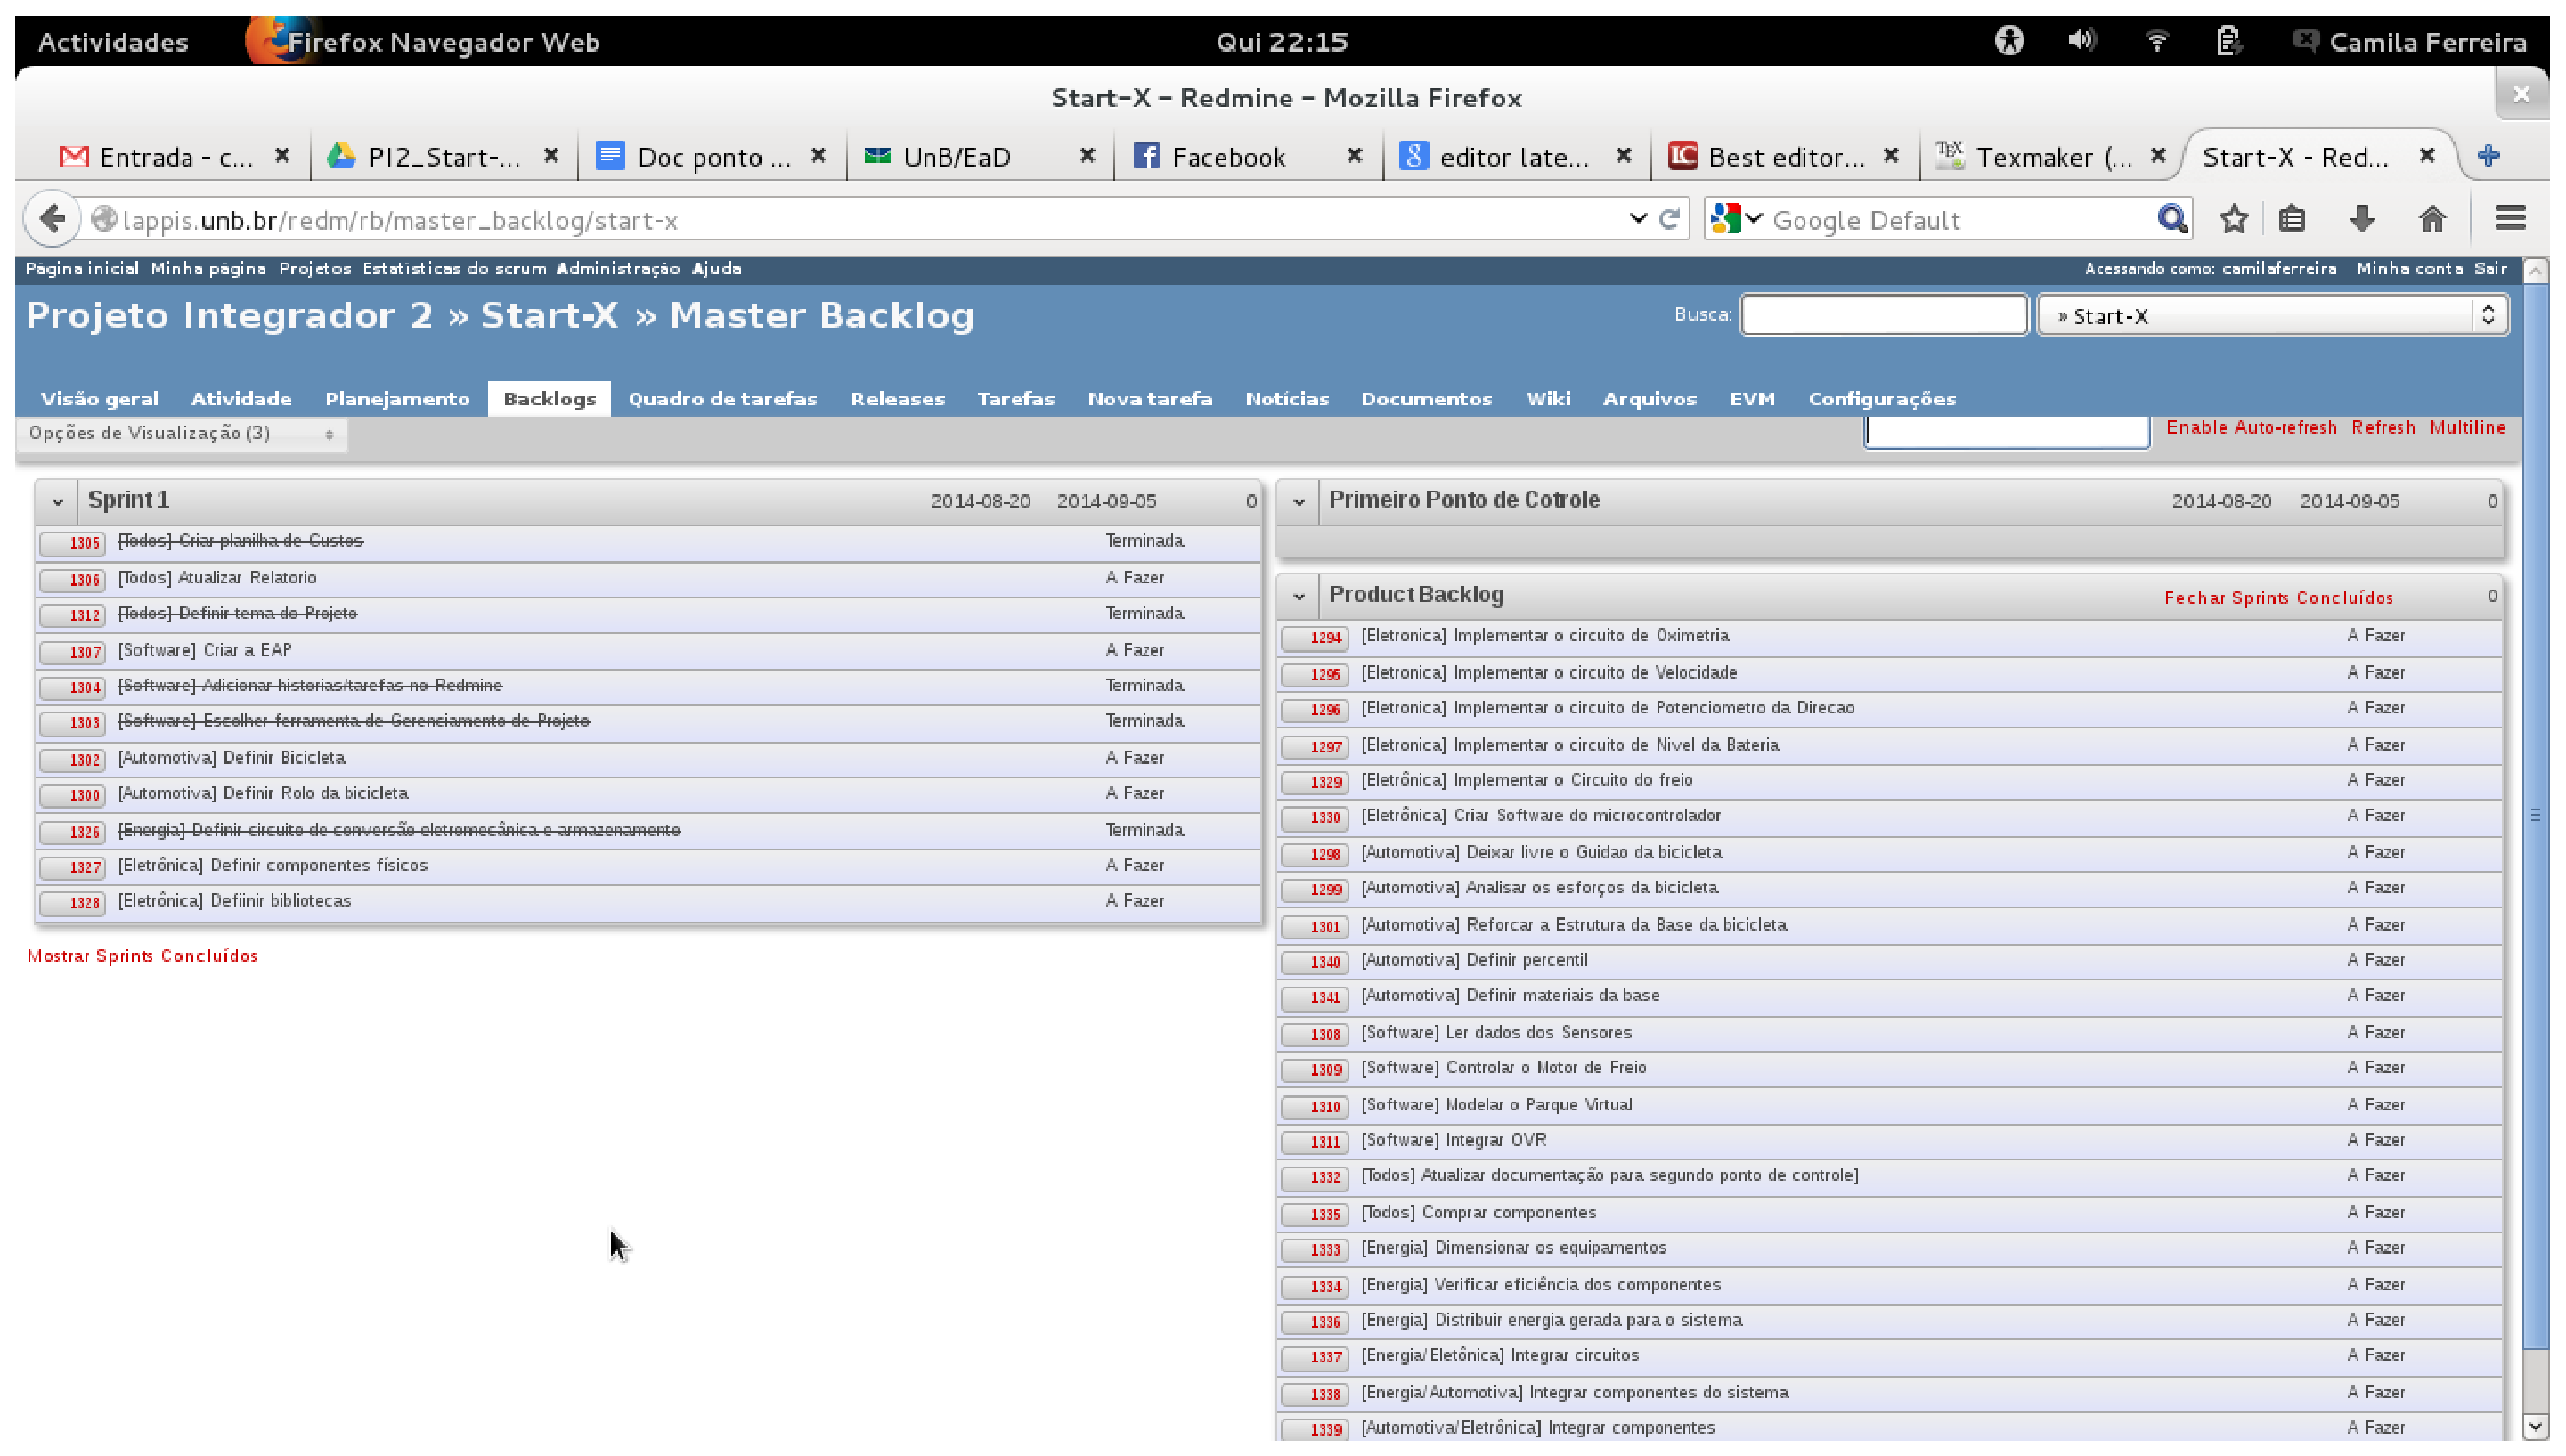
\includegraphics[width=0.8\textwidth]
      {figuras/backlogs.eps}
  \caption[redmine-backlog]
  \label{Redmine e backlog do projeto}
\end{figure}

Para gerir o projeto dividimos o projeto em 3 grandes releases que correspondem com os 3 pontos de controle que teremos duante o semestre. A primeira release se iniciou no primeiro dia de aula de Projeto Integrador 2 e termina no dia do primeiro ponto de controle; a segunda release se iniciará logo após a data do segundo ponto de controle e e terminará no dia do segundo ponto de controle e a terceira relase se iniciará logo após o segundo ponto de controle terminando no dia da entrega final do produto.

\begin{figure}[h]
  \centering
  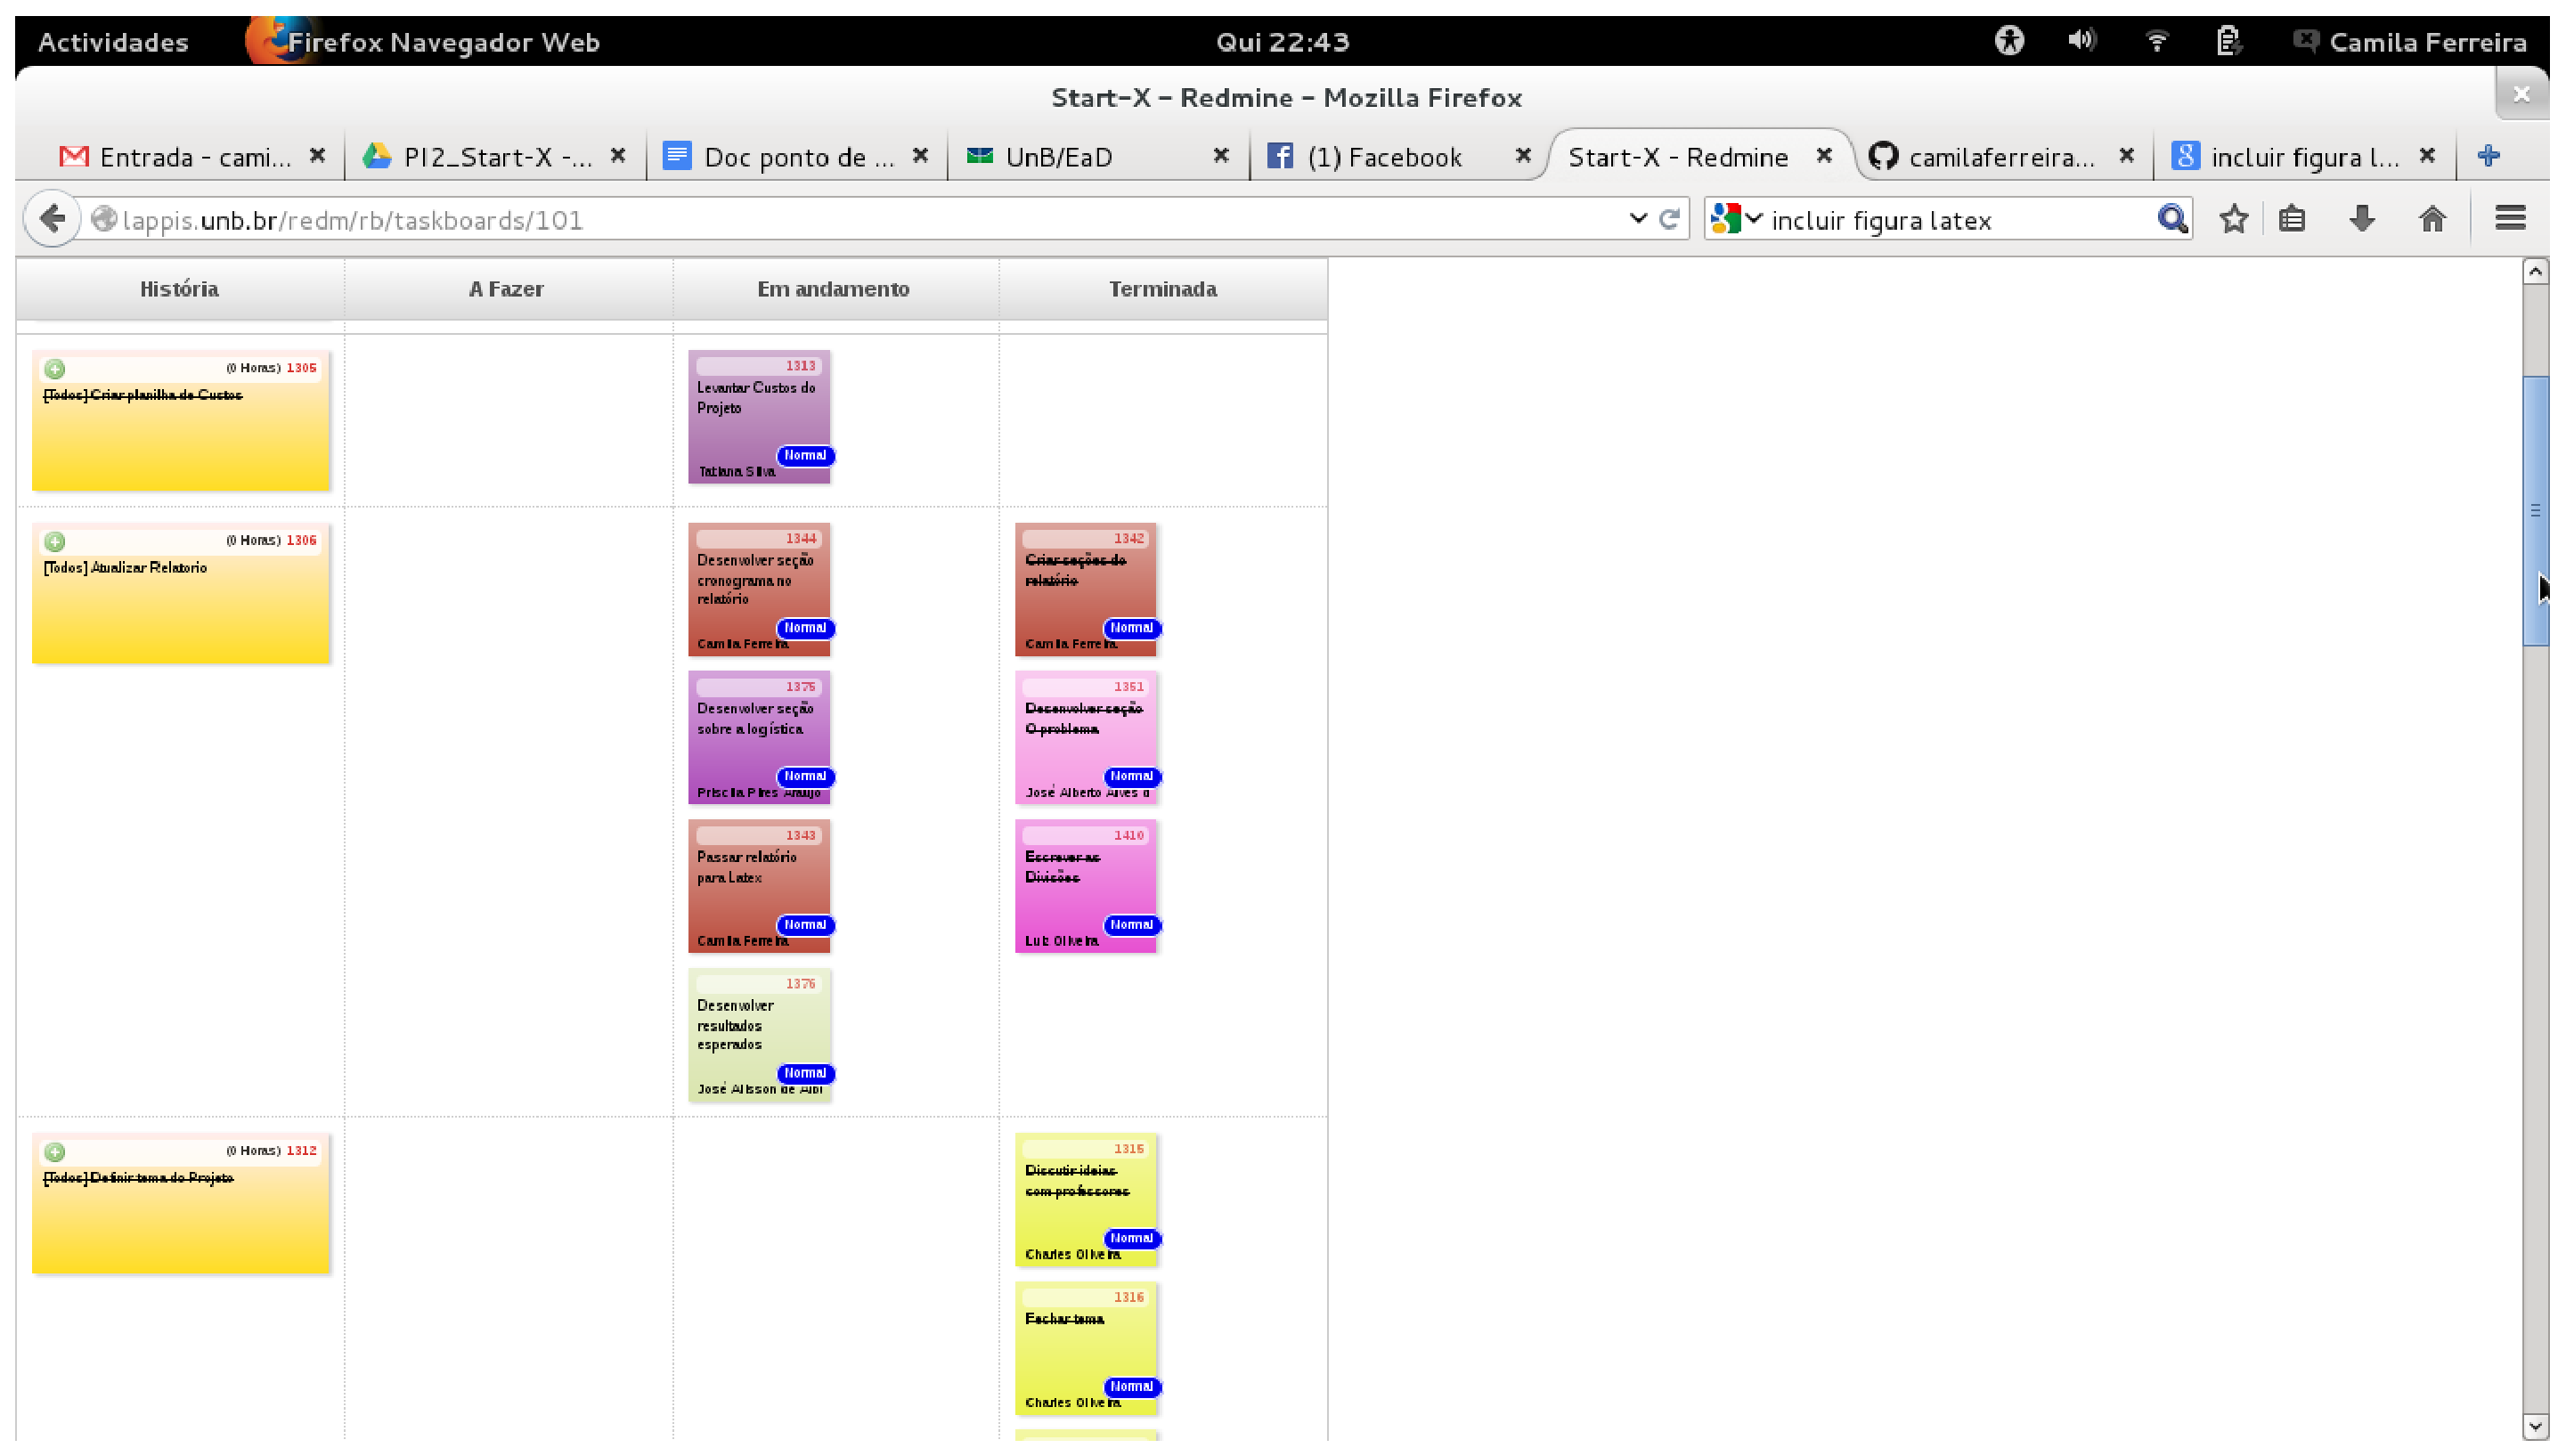
\includegraphics[width=0.8\textwidth]
      {figuras/quadrotarefas.eps}
  \caption[quadro-de-tarefas]
  \label{Quadro de tarefas}
\end{figure}
Para organizar as tarefas do projeto criamos histórias que são macrotarefas onde são posteriormente quebradas em tarefas menores. Essas tarefas são colocadas em um quadro de tarefas.


  

\chapter[Metas]{Metas}

Foram definidas 3 metas para o projeto:

\begin{itemize}
\item Definição do Projeto:
\begin{itemize}
	\item Definição do projeto e entrega do escopo.
\end{itemize}
\item Módulos funcionando separadamente:
\begin{itemize}
	\item  Os módulos do produto devem estar funcionando separadamente.
\end{itemize}
\item Produto concluído
\begin{itemize}
	\item A entrega do produto final com todos os módulos integrados e funcionais.
\end{itemize}
\end{itemize}

\chapter[Financeiro]{Financeiro}
Foi feita estimativa dos custos do projeto em termos de recursos materiais. Os custos relativos à recursos humanos serão calculados e apresentados nos próximos relatórios.

\begin{table}[htbp]
\resizebox{\columnwidth}{!}{%
\begin{tabular}{|p{2.5cm}|p{4.5cm}|p{4.5cm}|p{2.5cm}|p{4.5cm}|}
\hline
\multicolumn{ 5}{|c|}{\textbf{Tabela de custos do projeto}} \\ \hline\hline
\multicolumn{1}{|p{2.5cm}|}{\textbf{Áreas}} & \multicolumn{1}{p{5cm}|}{\textbf{Descrição das etapas}} & \multicolumn{1}{p{4.5cm}|}{\textbf{Materiais}} & \multicolumn{1}{p{2.5cm}|}{\textbf{Quantidade}} & \textbf{Valores} \\ \hline \hline
\multicolumn{ 1}{|p{2.5cm}|}{\textbf{Engenharia Automotiva}} & \multicolumn{ 1}{p{5cm}|}{Compra da bicicleta, após definição do usário} & \multicolumn{ 1}{p{4.5cm}|}{Bicicleta} & \multicolumn{ 1}{p{4.5cm}|}{1 unidade} & \multicolumn{ 1}{p{4.5cm}|}{R\$140.00} \\ 
\multicolumn{ 1}{ |p{2.5cm}|}{} & \multicolumn{ 1}{p{5cm}|}{} & \multicolumn{ 1}{p{4.5cm}|}{} & \multicolumn{ 1}{p{4.5cm}|}{} & \multicolumn{ 1}{p{4.5cm}|}{} \\ \cline{ 2- 5}
\multicolumn{ 1}{ |p{2.5cm}|}{} & \multicolumn{ 1}{p{5cm}|}{Construção do suporte para bicicleta} & Barra de aço chato 1020 & \multicolumn{1}{p{4.5cm}|}{2 metros} & R\$24.00 \\ \cline{ 3- 5}
\multicolumn{ 1}{ |p{2.5cm}|}{} & \multicolumn{ 1}{p{5cm}|}{} & Barra de aço retang. 1020 & \multicolumn{1}{p{4.5cm}|}{2 metros} & R\$30.00 \\ \cline{ 3- 5}
\multicolumn{ 1}{ |p{2.5cm}|}{} & \multicolumn{ 1}{p{5cm}|}{} & Barra de aço circular 1020 & \multicolumn{1}{p{4.5cm}|}{1 metros} & R\$14.00 \\ \cline{ 3- 5}
\multicolumn{ 1}{ |p{2.5cm}|}{} & \multicolumn{ 1}{p{5cm}|}{} & Rolamento de alumínio (rolo) & \multicolumn{1}{p{4.5cm}|}{1 unidade} & R\$70.00 \\ \cline{ 2- 5}
\multicolumn{ 1}{ |p{2.5cm}|}{} & \multicolumn{ 1}{p{5cm}|}{Peças para encaixe da roda traseira} & Conjunto de parafusos/rosca/porcas & \multicolumn{1}{p{4.5cm}|}{x} & R\$40.00 \\ \cline{ 3- 5}
\multicolumn{ 1}{ |p{2.5cm}|}{} & \multicolumn{ 1}{p{5cm}|}{} & Manípulo de Aperto Amaciador & \multicolumn{1}{p{4.5cm}|}{2 unidades} & R\$10.00 \\ \cline{ 3- 5}
\multicolumn{ 1}{ |p{2.5cm}|}{} & \multicolumn{ 1}{p{5cm}|}{} & Borracha para fixação & \multicolumn{1}{p{4.5cm}|}{4 unidades} & R\$30.00 \\ \cline{ 2- 5}
\multicolumn{ 1}{ |p{2.5cm}|}{} & \multicolumn{1}{p{5cm}|}{Junção das barras para o suporte} & Soldagem & \multicolumn{1}{p{4.5cm}|}{x} & R\$60.00 \\ \hline
\textbf{} &  &  &  &  \\ \hline
 & \textbf{Subtotal} & \textbf{} & \textbf{} & \textbf{R\$418.00} \\ \hline
 % &  &  &  &  \\ \hline
 &  &  &  &  \\ \hline\hline
\multicolumn{ 1}{|p{2.5cm}|}{\textbf{Engenharia Eletrônica}} & \multicolumn{ 1}{p{5cm}|}{Leitura da velocidade do ciclista} & Circuito & \multicolumn{1}{p{4.5cm}|}{1 unidade} & R\$3.00 \\ \cline{ 3- 5}
\multicolumn{ 1}{ |p{2.5cm}|}{} & \multicolumn{ 1}{p{5cm}|}{} & Sensor de velocidade & \multicolumn{1}{p{4.5cm}|}{1 unidade} & R\$170.00 \\ \cline{ 2- 5}
\multicolumn{ 1}{ |p{2.5cm}|}{} & \multicolumn{ 1}{p{5cm}|}{Leitura dos batimentos cardíacos do ciclista} & Circuito & \multicolumn{1}{p{4.5cm}|}{1 unidade} & R\$3.00 \\ \cline{ 3- 5}
\multicolumn{ 1}{ |p{2.5cm}|}{} & \multicolumn{ 1}{p{5cm}|}{} & Sensor de oximetria & \multicolumn{1}{p{4.5cm}|}{1 unidade} & R\$10.00 \\ \cline{ 2- 5}
\multicolumn{ 1}{ |p{2.5cm}|}{} & \multicolumn{1}{p{5cm}|}{Leitura do nível da bateria} & Sensor de nível de bateria & \multicolumn{1}{p{4.5cm}|}{1 unidade} & R\$10.00 \\ \cline{ 2- 5}
\multicolumn{ 1}{ |p{2.5cm}|}{} & \multicolumn{1}{p{5cm}|}{Medir o giro do guidão} & Potenciômetro p/ guidão & \multicolumn{1}{p{4.5cm}|}{1 unidade} & R\$1.00 \\ \cline{ 2- 5}
\multicolumn{ 1}{ |p{2.5cm}|}{} & \multicolumn{1}{p{5cm}|}{Leitor dos sensores} & 1 micro msp 430 & \multicolumn{1}{p{4.5cm}|}{1 unidade} & R\$30.00 \\ \cline{ 2- 5}
\multicolumn{ 1}{ |p{2.5cm}|}{} & \multicolumn{1}{p{5cm}|}{Frenar a bicicleta} & Servo motor & \multicolumn{1}{p{4.5cm}|}{1 unidade} & R\$40.00 \\ \cline{ 2- 5}
\multicolumn{ 1}{ |p{2.5cm}|}{} & \multicolumn{1}{p{5cm}|}{Ventilação do ciclista} & Cooler & \multicolumn{1}{p{4.5cm}|}{2 unidade} & R\$100.00 \\ \hline
 &  &  &  &  \\ \hline
 & \textbf{Subtotal} &  &  & \textbf{R\$367.00} \\ \hline
 % &  &  &  &  \\ \hline
 &  &  &  &  \\ \hline \hline
\multicolumn{ 1}{|p{2.5cm}|}{\textbf{Engenharia de Energia}} & \multicolumn{1}{p{5cm}|}{Transforma energia mecânica em elétrica} & Alternador & \multicolumn{1}{p{4.5cm}|}{1 unidade} & R\$230.00 \\ \cline{ 2- 5}
\multicolumn{ 1}{ |p{2.5cm}|}{} & \multicolumn{1}{p{5cm}|}{Armazenamento de energia} & No break (bateria, tomadas e inversor) & \multicolumn{1}{p{4.5cm}|}{1 unidade} & R\$260.00 \\ \cline{ 2- 5}
\multicolumn{ 1}{ |p{2.5cm}|}{} & \multicolumn{1}{p{5cm}|}{Medição} & Multímetro & \multicolumn{1}{p{4.5cm}|}{2 metros} & R\$40.00 \\ \cline{ 2- 5}
\multicolumn{ 1}{ |p{2.5cm}|}{} & \multicolumn{ 1}{p{5cm}|}{Distribuição de energia} & Cabos (chicotes) & \multicolumn{1}{p{4.5cm}|}{1 unidade} & R\$18.00 \\ \cline{ 3- 5}
\multicolumn{ 1}{ |p{2.5cm}|}{} & \multicolumn{ 1}{p{5cm}|}{} & Cabos tipo jacaré & \multicolumn{1}{p{4.5cm}|}{4 unidade} & R\$16.00 \\ \hline
 &  &  &  &  \\ \hline
 & \textbf{Subtotal} &  &  & \textbf{R\$564.00} \\ \hline
 % &  &  &  &  \\ \hline
 &  &  &  &  \\ \hline \hline
\multicolumn{ 1}{|p{2.5cm}|}{\textbf{Engenharia de Software}} & \multicolumn{ 1}{p{5cm}|}{Óculos usado para simular ambiente virtual} & \multicolumn{ 1}{p{4.5cm}|}{Oculus Rift} & \multicolumn{ 1}{p{4.5cm}|}{1 undiade} & \multicolumn{ 1}{p{4.5cm}|}{R\$1,500.00} \\ 
\multicolumn{ 1}{ |p{2.5cm}|}{} & \multicolumn{ 1}{p{5cm}|}{} & \multicolumn{ 1}{p{4.5cm}|}{} & \multicolumn{ 1}{p{4.5cm}|}{} & \multicolumn{ 1}{p{4.5cm}|}{} \\ \hline
 &  &  &  &  \\ \hline
 & \textbf{Subtotal} &  &  & \textbf{R\$1,500.00} \\ \hline
 % &  &  &  &  \\ \hline
 &  &  &  &  \\ \hline \hline
 & \textbf{Total} &  &  & \textbf{R\$2,849.00} \\ \hline
\end{tabular}
}
\caption{Planilha de custos com equipamentos/materiais}
\label{fabela_fudida}
\end{table}

Considerando o valor médio ganho por um estagiário de Engenharia como 900,00 reais,
com 20 horas semanais temos que uma hora de um estagiário de engenharia equivale a
11,25 reais.

Consideramos 6 horas de trabalho por semana em 16 semanas dedicadas ao projeto Start-X.

\begin{table}[h]
\centering
\begin{tabular}{|l|c|l|}
\hline
Integrante       & \multicolumn{1}{l|}{Horas Trabalhadas} & Valor Total \\ \hline
Camila Ferreira  & 96                                     & R\$1,080     \\ \hline
Charles Daniel   & 96                                     & R\$1,080     \\ \hline
Gabriela Navarro & 96                                     & R\$1,080     \\ \hline
José ALberto     & 96                                     & R\$1,080     \\ \hline
José Alisson     & 96                                     & R\$1,080     \\ \hline
Júlio Cezar      & 96                                     & R\$1,080     \\ \hline
Lucas Kanashiro  & 96                                     & R\$1,080     \\ \hline
Luiz Fernando    & 96                                     & R\$1,080     \\ \hline
Macarcur Sousa   & 96                                     & R\$1,080     \\ \hline
Priscila Pires   & 96                                     & R\$1,080     \\ \hline
Tatiana Dias     & 96                                     & R\$1,080     \\ \hline
Thiago Ferreira  & 96                                     & R\$1,080     \\ \hline
\multicolumn{2}{|r|}{Total}                               & R\$12,960    \\ \hline
\end{tabular}
\caption{Planilha de custos com pessoal.}
\end{table}

Custo Total

\begin{table}[h]
\centering
\begin{tabular}{|l|l|}
\hline
Tipos de custo              & Valor       \\ \hline
Equipamentos/materiais      & R\$2,849.00 \\ \hline
Pessoal                     & R\$12,960   \\ \hline
\multicolumn{1}{|r|}{Total} & R\$15,809   \\ \hline
\end{tabular}
\caption{Custo total do projeto}
\end{table}


 
 

\part{Desenvolvimento}
Este capítulo descreve partes do sistema como um todo, abrangendo ferramentas de controle de estrutura, módulos de interface, hardwares envolvidos e afins. Serão apresentados os desenvolvimentos das partes de:

\begin{itemize}
	\item \nameref{software}
	\begin{itemize}
		\item Controle de infraestrutura
		\item Interface de controle
		\item Visualização de dados
	\end{itemize}
	\item \nameref{eletrônica}
	\begin{itemize}
		\item Aquisição de dados
		\begin{itemize}
			\item Circuito do sistema
			\item Interface de aquisição e disponibilização dos dados (microcontrolador)
		\end{itemize}
	\end{itemize}
	\item \nameref{automotiva}
	\begin{itemize}
		\item Estrutura do produto e seus esforços
	\end{itemize}
	\item \nameref{energia}
	\begin{itemize}
		\item Acoplamento do alternador
		\item Cálculos de eficiência
	\end{itemize}
\end{itemize}


\chapter{Software}
\label{software}

\section{Puppet} % (fold)
\label{sec:puppet}

Para agilizar e evitar os problema com compatibilidades e erros de versões de bibliotecas e outros ativos, foi utilizado a ferramenta \href{http://puppetlabs.com}{Puppet} para auxiliar com este processo administrativo de desenvolvimento do sistema. O Puppet está sendo usado como ferramanta para gerenciamento de configuração do ambiente de desenvolvimento do projeto Bike-X.

\subsection{O que é o Puppet} % (fold)
\label{sub:o_que_o_puppet}

\gls{puppet} é uma ferramenta de gerenciamento de configuração feita em \gls{ruby} que permite que seja definido o estado da infraestrutura de TI (Tecnologia da Informação), com isso, a configuração pode ser replicada em qualquer ambiente, levando em consideração as restrições de implementação da definição do ambiente. Para gerenciamento de alguns servidores ou maquinas, sejam elas físicas ou virtuais, o Puppet automatiza as tarefas administrativas do sistema que normalmente são feitas manualmente, liberando tempo e espaço mental dos administradores de sistemas para trabalhar nos projetos que proporcionam maior valor ao negócio.

O Puppet possui uma sintaxe própria, o mesmo utiliza uma linguagem declarativa, ao invés de uma linguagem imperativa, que é utilizada pela maioria das ferramentas similares, como por exemplo o \gls{chef}. A linguagem imperativa é um conceito baseado em estados, definidos por variáveis, e ações que são manipuladoras de estado, procedimentos. Pelo fato de permitir o uso de procedimentos como estruturação, também é conhecido como procedural. A linguagem declarativa, ao contrário da linguagem imperativa que informa ao computador "como" as instruções devem ser executadas, preocupa-se em apenas dizer ao computador "o que" precisa ser feito, cabendo ao computador decidir qual a melhor solução para essa solicitação.
 

\subsection{Integrando o Puppet ao projeto} % (fold)
\label{sub:integrando_o_puppet_ao_projeto}

Para a utilização do Puppet dentro do projeto foi desenvolvido um módulo puppet específico, chamado \href{https://github.com/start-x/startx-src/tree/master/puppet}{bike-x}. Nesse módulo é definido nome e versão de pacotes a serem instalados, é definido links simbólicos, criação de arquivos de configuração para o \gls{rift}. O módulo em questão foi testado e homologado para algumas distribuições do sistema operacional Linux:

\begin{itemize}
\item Ubuntu 13.10
\item Ubuntu 14.04
\item Mint 17
\item Debian Wheezy
\item Debian Sid
\end{itemize}

Todas as distribuições apresentadas são "Debian like" e o módulo está totalmente modularizado para a adição de qualquer nova distribuição necessária, entretanto, as apresentadas acima atende 100\% a equipe de desenvolvimento do projeto. A lista de pacotes Debian necessários para o projeto estão listados a seguir:

\begin{multicols}{2}
\begin{itemize}
\item python2.7
\item python2.7-dev
\item python-serial
\item doxygen
\item graphviz
\item dots
\item binutils-msp430
\item gcc-msp430
\item msp430-libc
\item msp430mcu
\item mspdebug
\item libxext-dev
\item mesa-common-dev
\item freeglut3-dev
\item libxinerama-dev
\item libxrandr-dev
\item libxxf86vm-dev
\item swig
\end{itemize}
\end{multicols}

A seguir lista de pacotes Python utilizados:

\begin{itemize}
\item pyserial
\item mock
\end{itemize}

Após a execução do módulo Puppet desenvolvido, todos os pacotes listados acima estarão instalados no sistema. Para facilitar a execução do módulo Puppet para todos da equipe, foi desenvolvido um Shell script chamado "setup\_development\_environment.sh" onde é instalado o Puppet em si e os módulos que são dependência, que são o \textit{pip} e \textit{stdlib}, e executado o módulo Puppet bike-x.



\section{Sistema BikeX}
\label{sec:sistema_bikex}

%Software Bikex: modelagem (uml), linguagem, signals, arquitetura
\subsection{Módulos}
Esta seção visa descrever como os diversos módulos do sistema irão se comportar separadamente e como vão interagir entre si. O sistema será composto pelos Unity, Bikex, Device. A figura \ref{diagrama-classes} exemplifica como os módulos interagem entre si.

O módulo Unity será responsável com as interações entre o usuário e o sistema. A primeira responsabilidade é retornar para o sistema a altitude atual do usuário. Essa informação será usada para definir se é necessário o acionamento da frenagem para simular uma inclinação no ambiente virtual. Outra responsabilidade será definir a posição e rotação atual do usuário no sistema. Essas informações irão ser disponibilizadas com a interação de outros módulos. Algumas informações serão disponibilizadas pelo sistema para o usuário. Informações como: velocidade, distância e a velocidade máxima atingida pelo usuário. Por fim, esse módulo irá fazer a renderização do frame para o usuário. Essa renderização irá considerar todas as interações com o sistema e as informações geradas com essa interação.

\begin{figure}[h]
  \centering
	%\includegraphics[scale=0.5]{figuras/diagrama_de_classe}
  \caption{Diagrama de classes}
  \label{diagrama-classes}
\end{figure}

No sistema terá um módulo que será composto por várias classes. Esse módulo, que é o responsável em fazer a interação com os dispositivos externos, se chama Device. Primeiramente, a classe principal será uma interface chamada Device. Duas classes irão relacionar com essa interface diretamente, a Active e a Passive. A classe Active representará os dispositivos que irão influenciar ativamente e fisicamente no sistema. Essa classe irá ser responsável por informar os dados para essa influência no sistema. Um dispositivo que exemplificar é a frenagem do sistema. A classe Passive são dispositivos que fornecem informações para o sistema. Os dispositivos de velocidade, direção e OVR são exemplos desse tipo de Device. A classe Passive irá ser responsável de coletar informações desses dispositivos e fornecer para o sistema realizar os procedimentos necessários. O dispositivo OVR é o Oculus em si e será responsável em fornecer a posição da cabeça do usuário.

O módulo Bikex é o módulo central do sistema e fará a interface com o módulo Unity e os outros módulos. Esse módulo é responsável por receber as informações dos dispositivos do tipo Passive e fazendo as transformações necessárias para enviar para o módulo Unity. O primeiro procedimento que esse módulo realiza é o cálculo da posição do usuário e tem como entrada a velocidade e a direção atuais do usuário. Outro procedimento será o cálculo da rotação do usuário. Isso será feito a partir de dados fornecidos pelo dispositivo Oculus. Essa rotação definirá a direção que o usuário está olhando. Definimos a separação desses dois procedimentos para que a rotação da cabeça do usuário não interfira na rotação da bicicleta. O outro procedimento é definir a intensidade de frenagem de acordo com a altitude coletada do módulo Unity. A partir dessa intensidade, o Bikex aciona o dispositivo de freio com a mesma.



%Unity: scripts, modelagem, assets etc
\subsection{Unity}

%Python: versao do python, modulos puppet, modulos para comunicacao UART
\subsection{Python}

%Falar aqui sobre o software do bikex, a integracao do python/msp430/unity
\subsection{Integração Sensores e Sistema}

\section{Funcionamento do Oculus Rift}
Colocar aqui como o Oculus Rift define os valores gerados, como eh feita a distorcao, como eh feito o calculo de customizacao para pessoas com diferentes distancia entre os olhos e talz

\subsection{Esquema de coordenadas}
Falar do esquema de coordenadas do Oculus rift. Traduzir:
As seen from the diagram, the coordinate system uses the follow-
ing axis definitions:
\begin{itemize}
	\item Y eh positivo para cima
	\item X eh positivo para direita
	\item Z eh positivo para tras
\end{itemize}
Rotation is maintained as a unit quaternion, but can also be
reported in yaw-pitch-roll form. Positive rotation is counter-
clockwise (CCW, direction of the rotation arrows in the diagram)
when looking in the negative direction of each axis, and the com-
ponent rotations are:
\begin{itemize}
	\item Pitch is rotation around X, positive when pitching up.
	\item Yaw is rotation around Y , positive when turning left.
	\item Roll is rotation around Z, positive when tilting to the left in the XY plane.
\end{itemize}

\begin{figure}[h]
  \centering
  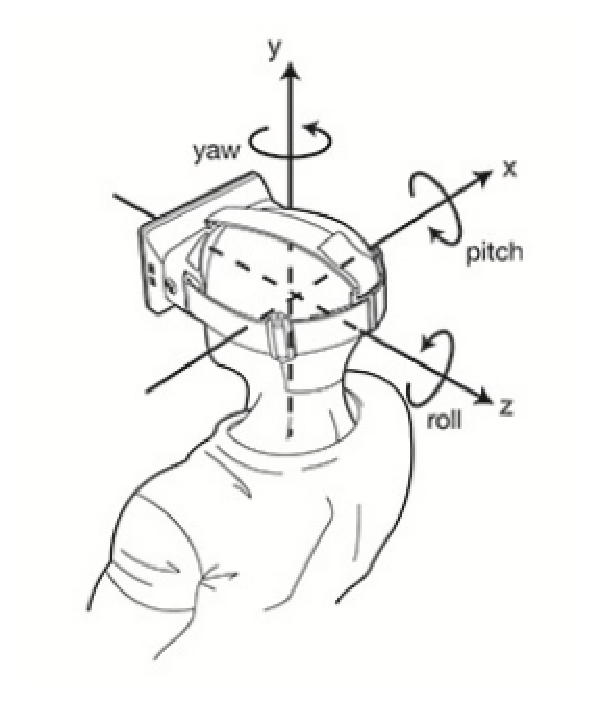
\includegraphics[width=0.5\textwidth]
      {figuras/esquema_coordenadas_rift.eps}
  \caption{Esquema de coordenadas do Oculus Rift}
  \label{coordenadas-rift}
\end{figure}

\subsection{Distorcao}
Falar aqui um pouco sobre as distorcoes da lente e das imagens. Traduzir:
The Oculus Rift requires the scene to be rendered in split-screen stereo with half the screen used for each
eye. When using the Rift, the left eye sees the left half of the screen, and the right eye sees the right half.
Although varying from person-to-person, human eye pupils are approximately 65 mm apart. This is known
as interpupillary distance (IPD). The in-application cameras should be configured with the same separation.
Note that this is a translation of the camera, not a rotation, and it is this translation (and the parallax effect
that goes with it) that causes the stereoscopic effect. This means that your application will need to render the
entire scene twice, once with the left virtual camera, and once with the right.
Note that the reprojection stereo rendering technique, which relies on left and right views being generated
from a single fully rendered view, is usually not viable with an HMD because of significant artifacts at object
edges.
The lenses in the Rift magnify the image to provide a very wide field of view (FOV) that enhances immersion.
However, this process distorts the image significantly. If the engine were to display the original images on the
Rift, then the user would observe them with pincushion distortion.
To counteract this distortion, the software must apply post-processing to the rendered views with an equal
and opposite barrel distortion so that the two cancel each other out, resulting in an undistorted view for each
eye. Furthermore, the software must also correct chromatic aberration, which is a rainbow effect at the edges
caused by the lens. Although the exact distortion parameters depend on the lens characteristics and eye
position relative to the lens, the Oculus SDK takes care of all necessary calculations when generating the
distortion mesh.
When rendering inside the Rift, projection axes should be parallel
to each other as illustrated in Figure 5, and the left and right views
are completely independent of one another. This means that
camera setup is very similar to that used for normal non-stereo
rendering, except that the cameras are shifted sideways to adjust
for each eye location.
In practice, the projections in the Rift are often slightly off-center
because our noses get in the way! But the point remains, the left
and right eye views in the Rift are entirely separate from each
other, unlike stereo views generated by a television or a cinema
screen. This means you should be very careful if trying to use
methods developed for those media because they do not usually
apply to the Rift.
Figure 5: HMD eye view cones.
The two virtual cameras in the scene should be positioned so that they are pointing in the same direction
(determined by the orientation of the HMD in the real world), and such that the distance between them is the
same as the distance between their eyes, or interpupillary distance (IPD). This is typically done by adding the
ovrEyeRenderDesc::ViewAdjust translation vector to the translation component of the view matrix.
Although the Rift’s lenses are approximately the right distance apart for most users, they may not exactly
match the user’s IPD. However, because of the way the optics are designed, each eye will still see the correct
view. It is important that the software makes the distance between the virtual cameras match the user’s IPD
as found in their profile (set in the configuration utility), and not the distance between the Rift’s lenses.

\begin{figure}[h]
  \centering
  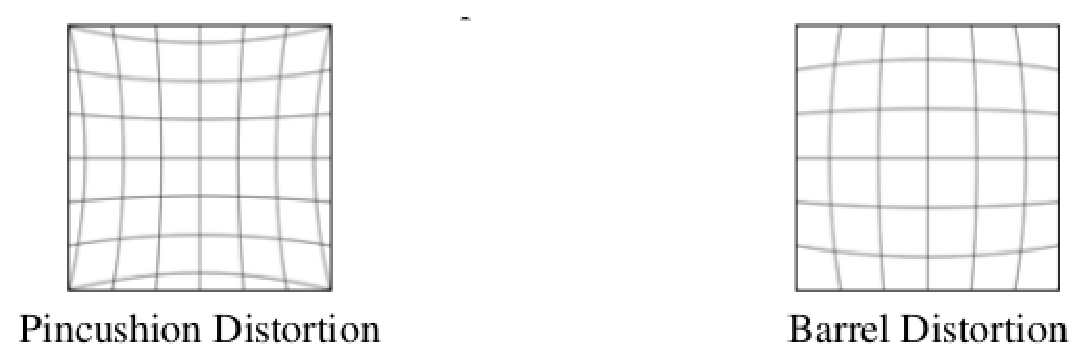
\includegraphics[width=0.7\textwidth]
      {figuras/distorcao_rift.eps}
  \caption{Distorcao de lentes e imagens do Rift}
  \label{coordenadas-rift}
\end{figure}


\section{Unity 3D} % (fold)
\label{sec:unity_3d}

\subsection{O Unity }
\label{sub:o_unity}
	A unidade é um IDE de desenvolvimento de jogos com um potente mecanismo de renderização e totalmente integrado com um conjunto de ferramentas que permitem criação de conteúdos interativos em varias plataformas e em  3d ou 2d.Além disso é possivel gerar builds para de 16 plataformas  como o linux , android ,windows e iOS com um alto nivel de qualidade pois é possível utilizar recursos prontos da Assert Store e de comunidades de compartilhamento de conhecimentos. 
	Para esse projeto foi escolhido o Unity pois  além dos benefícios citados acima com ele é possível que o desenvolvimento seja mais agil, em menos tempo e com umcusto menor e com uma qualidade razoável. 

\subsection{Workflow} % (fold)
\label{sub:workflow}
	Com o intuito de simplificar o processo de criação e produção de software, o Unity oferece um ambiente de trabalho com diversas ferramentas integradas para o desenvolvimento para a possibilitar a criação de mundos complexos com bloco de construção de cenas rapidamente escaláveis, implementar fluxos de controle utilizando linguagens altamente utilizadas no mercado como C\# e Java Script, com uma perfomace de tempo de compilação. Além disso durante o processo de criação é possível economizar tempo utilizando elementos prontos, salas e forúm de bate papo para distribuição de conhecimentos e resolução de problemas e dúvidas.

\begin{figure}[h]
  \centering
  \includegraphics[width=0.8\textwidth]
      {figuras/bike.png}
  \caption{Edição de objeto no Unity}
  \label{coordenadas-rift}
\end{figure}

\subsection{Modelagem de Elementos} % (fold)
\label{sub:modelagem}
	Para a utilização de elementos no Unity é necessario a criação de objetos 3d, para isso pode ser utilizado qualquer um das IDE mais utilizadas do mercado tais como Maya , 3DMax, Blender ,Cinema4D, Modo, Lightwave, Cheetah3D, entre outros. A manipulação e ajustes de objetos em 3D está sendo realizada através da utilização da ferramenta blender  que é uma plataforma livre de alto desempenho que permite além da modelagem para a criação de objetos 3D e contém ferramentas para animações, criação de jogos, construção de foto realismo, simulações de fluidos, edição de vídeos,entre outros.Depois de feito os ajustes nos modelos o Blender possui suporte para exportar objetos nos formatos de arquivo: 3DS,DXF,FBX,OBJ,LWO,SVG,STL entre outros.

\begin{figure}[h]
  \centering
  \includegraphics[width=0.8\textwidth]
      {figuras/blender.png}
  \caption{Renderização de \textit{Bick Buck Bunny} sendo feita no Blender}
  \label{coordenadas-rift}
\end{figure}

\subsection{SDK OculusVR}
\label{sub:sdk_ovr}
      Nos primeiros passos para a integração do Oculus Rift com o Unity foi necessário a utilização de uma SDK\footnote{ SDK encontrada em \url{https://developer.oculusvr.com/?action=dl&v=8 }} do próprio Oculus Rift ,que atualmente possui as versões 0.2, 0.3 e 0.4, que permite extrair dados do oculus e manipulos utilizando C++. No entanto como o Unity possui suporte para o plugin do Oculus Rift, que são scripts oriundos da SDK que ao invés de ser implementada em C++ é implementada em C\#, foi adotado o mesmo para auxiliar no controle do ambiente virtual no Unity.

\subsection{Criação de Scripts}
\label{sub:criacao_de_scripts}







\section{Ambiente virtual}
	Para iniciar a modelagem do Parque Virtual foi escolhido um mapa em escala de 
cinza para que sirva de base para a montagem do terreno do ambiente virtual.Para isso 
qualquer editor de imagem pode ser utilizado , no caso do projeto foi utilizado o photoshop,
e a imagem foi tratada e exportada para o formato aceito pelo Unity que é o 'RAW' . Abaixo estão 
as imagens do arquivo do ambiente virtual em escala de cinza e o ambiente virtual que foi gerado.

\begin{figure}[htpb]
 \begin{center}
    \includegraphics[width=.40\textwidth]{figuras/mapa_escala_de_cinza.jpg}
 \end{center}
  \caption{Mapa do ambiente virtual em escala de cinza}
  \label{fig:core_concurrent}
\end{figure}

\begin{figure}[htpb]
 \begin{center}
    \includegraphics[width=.60\textwidth]{figuras/mapa.png}
 \end{center}
  \caption{Mapa do ambiente virtual gerado e modificado}
  \label{fig:core_concurrent}
\end{figure}

O mapa foi importado para o Unity e foi colocada nele uma base de grama para que
os outros componentes sejam colocadas por cima desta base.Foi feita uma adequação 
do terreno formado pelo mapa de cores para que fosse criada
a ciclovia e na parte mais baixa do mapa foi adicionado água para termos pequenos 
lagos.

Os elementos que estão sendo adicionados no conforme idéias e necessidades encontradas
pela equipe, primeiramente inserimos algumas árvores e vegetações para dar uma visão
de parque ao mapa, inserimos também uma ponte para que o usuário possa passar por um 
ponto de água, está sendo elaborado um túnel para que o usuário possa passar e uma 
cachoeira para ser admirada durante o passeio no ambiente. Para uma melhor visualização 
dos ambiente que estarão no ambiente virtual abaixo estão algumas imagens tiradas do ambiente
 no processo de montagem usando o unity.

\begin{figure}[htpb]
 \begin{center}
    \includegraphics[width=.60\textwidth]{figuras/bicycle.png}
 \end{center}
  \caption{Bicicleta utilizada pelo usuário no ambiente virtual}
  \label{fig:core_concurrent}
\end{figure}

\begin{figure}[htpb]
 \begin{center}
    \includegraphics[width=.60\textwidth]{figuras/bridge.png}
 \end{center}
  \caption{Ponte para uma atravessia no lago}
  \label{fig:core_concurrent}
\end{figure}

\begin{figure}[htpb]
 \begin{center}
    \includegraphics[width=.60\textwidth]{figuras/farm.png}
 \end{center}
  \caption{Fazenda criada em uma área do ambiente virtual}
  \label{fig:core_concurrent}
\end{figure}

\begin{figure}[htpb]
 \begin{center}
    \includegraphics[width=.60\textwidth]{figuras/tunel1.png}
 \end{center}
  \caption{Visão 1 do tunel gerado no ambiente virtual}
  \label{fig:core_concurrent}
\end{figure}

\begin{figure}[htpb]
 \begin{center}
    \includegraphics[width=.60\textwidth]{figuras/tunel2.png}
 \end{center}
  \caption{Visão 2 do tunel gerado no ambiente virtual}
  \label{fig:core_concurrent}
\end{figure}

\begin{figure}[htpb]
 \begin{center}
    \includegraphics[width=.60\textwidth]{figuras/tunel3.png}
 \end{center}
  \caption{Visão interior do tunel}
  \label{fig:core_concurrent}
\end{figure}

\begin{figure}[htpb]
 \begin{center}
    \includegraphics[width=.60\textwidth]{figuras/rock.png}
 \end{center}
  \caption{Visão de algumas pedras para dar mais realizadade ao ambiente}
  \label{fig:core_concurrent}
\end{figure}

\begin{figure}[htpb]
 \begin{center}
    \includegraphics[width=.60\textwidth]{figuras/waterfall.png}
 \end{center}
  \caption{Visão de uma Cachoeira}
  \label{fig:core_concurrent}
\end{figure}


\chapter{Eletrônica}
\label{eletronica}

\section{Microcontrolador} % (fold)
\label{sec:msp430}

% É um microcontrolador RISC de 16 bits criado pela Texas Instrumets para aplicações de baixo consumo de energia.
O microcontrolador utilizado neste projeto foi o MSP430G2553. Este microcontrolador possui uma arquitetura RISC com registradores de 16 \textit{bits} e 27 instruções, 512 \textit{Bytes} de RAM e pode operar com um \textit{clock} de até 16MHz. As aplicações foram trabalhadas a partir da plataforma MSP430 \textit{Launchpad}. Esta plataforma foi desenvolvida pela \textit{Texas Instruments} (TI) como um \textit{kit} de avaliação para microcontroladores da linha MSP430G. Este microcontrolador apresenta algumas características importantes para a realização deste trabalho. São elas:
\begin {itemize}
	\item 2 \textit{Timers} (TA0 e TA1) com 16 \textit{bits} e 4 modos de contagem;
	\item 8 canais de entrada para um Conversor A/D de 10\textit{bits} ( ADC10 tipo SAR);
	\item Serviços de interrupção por \textit{Hardware};
	\item \textit{Hardware} de comunicação serial com suporte para UART.
\end {itemize}

\begin{figure}[h]
  \centering
  \includegraphics[width=0.6\textwidth]
      {figuras/Launchpad.jpg}
  \caption{Pataforma para desenvolvimento MSP430 \textit{Launchpad}.}
  \label{Launchpad}
\end{figure}
% Colocar aqui sobre o que é o MSP430, sua função no projeto como foi utilizado
Em comparação com outras plataformas, como o Arduino, a MSP430 \textit{Launchpad} apresenta um menor custo. A plataforma Arduino apresenta mais facilidade para a implementação de protótipos através de sua linguagem de programação na Arduino IDE, porém, a plataforma \textit{Launchpad} também possuí uma plataforma similar disponível chamada de \textit{Energia}. Neste projeto, entretanto, optou-se por utilizar a ferramenta msp430-gcc e mspdebug para desenvolver as aplicações de software embarcado e programar o dispositivo respectivamente. Elas foram escolhidas por possibilitar mais liberdade de desenvolvimento no microcontrolador e possibilidade de seguir em nível mais próximo do \textit{hardware}, apesar da maior complexidade na elaboração das aplicações.


%\subsection{MSPGCC} % (fold)
%\label{sub:mspgcc}

%É um porte do \textit{GNU C Compiler} (\textbf{GCC}) e do \textit{GNU Binutils} (\textbf{as}, \textbf{ld}) para o microcontrolador \textit{MSP430}. São providenciadas ferramentas para depuração e \textit{download} de binário (\textbf{GDB, JTAG} e \textbf{BSL}).

% Item sobre a visão sistemica da eletronica embarcada

\subsection{Arduindo}
\label{sec:arduino}

O Arduino é plataforma \textit{open-source} criada de forma a facilitar o uso da integração de \textit{software} e \textit{hardware}. Foi utilizado o microcontrolador Arduino Mega que é baseado no Atmega 1280. Tem-se um total de 54 pinos digitais de entrada e saída no qual 14 deles tem a possibilidade de serem usados como um sinal PWM (\textit{Pulse Width Modulation}), 16 pinos para entrada de sinais analógicos, 4 portas para comunicação UART (\textit{Universal asynchronous receiver/transmitter}), um oscilador de cristal de 16 MHz, uma conexão USB, uma entrada de alimentação e um botão de \textit{reset}.

O ATmega1280 possui algumas características que foram importantes para a sua escolha como substituição do \textit{MSP430 Launchpad} 128 KB de memória \textit{flash} para armazenamento de código (dos quais 4KB são usados pelo \textit{bootloader}), 8 KB de SRAM e 4 KB de EEPROM (que poder ser lidos e escritos com a biblioteca EEPROM). Outras características importantes são a quantidade de portas de entrada e saída disponíveis, o que permitiu uma maior liberdade ao receber os sinais dos sensores; 

A programação foi realizada utilizando o ambiente de desenvolvimento (IDE) da plataforma Arduino que permite a programação em C/C++. Isto permite controlar e criar operações de entrada e saída dos sensores e do atuador.



\section{Visão Sistêmica da Eletronica Embarcada} % (fold)
\label{sec:visao_sistemica}

No ponto de vista da eletrônica embarcada, enxergam-se dois pontos principais: O PC com o ambiente virtual e os sensores e atuadores instalados na bicicleta. O primeiro destes realizará o processamento do ambiente virtual a partir dos dados obtidos pelos sensores e atualizando a posição do ciclista no ambiente. Em seguida, devolverá como sinal de retorno à bicicleta no controle do freio para transmitir uma sensação de peso ao ciclista. Para tornar isso possível, trabalhou-se com 2 sensores e um atuador, listados a seguir.


\begin {itemize}
	\item Posição do guidão;
	\item Velocidade da roda.
	\item Servo motor.
\end  {itemize}

Neste contexto, o sistema de software embarcado foi projetado baseando-se no diagrama de blocos apresentado na Figura \ref{blocos}. O sensor de posição do guidão se trata de um potenciômetro comum com variação de ângulo de 0 a 270 graus e 0 a 10 k$\Omega$ de variação de resistência proporcional ao ângulo. O sensor de velocidade se trata de um conta giros através de interferência entre um par transmissor-receptor de infravermelho que permitirá verificar o movimento da roda traseira. O atuador constante em um servomotor cuja posição será controlada de forma a controlar o freio da bicicleta, aumentando o atrito com a roda traseira e fornecendo uma sensação de peso ao usuário.

\begin{figure}[h]
  \centering
  \includegraphics[width=0.8\textwidth]
      {figuras/diag_blocos_elet1.png}
  \caption{Diagrama de blocos do sistema no ponto de vista do \textit{hardware} embarcado.}
  \label{blocos}
\end{figure}

% Item sobre o projeto de software embarcado
\section{Projeto do \textit{Software} Embarcado} % (fold)
\label{sec:soft_emb}
Visando facilitar o desenvolvimento do \textit{software} a ser embarcado no microcontrolador, implementou-se uma biblioteca contendo funções para o uso especifico no \textit{kit} \textit{Launchpad}, com botões, LEDs e portas de comunicação pré definidas. Essa biblioteca contem funções básicas para entradas e saídas digitais, \textit{timer} e comunicação. Outras duas bibliotecas são utilizadas neste projeto, sendo uma para amostrar um sinal a partir do conversor A/D e outra contendo as definições do ambiente virtual.
A principio, o projeto de \textit{software} foi direcionado a leitura dos sensores do guidão, velocidade, atuador e comunicação. A seguir, serão descritas as implementações destas etapas neste projeto.

\subsection{Leitura de posição do guidão} % (fold)
\label{sub:read_guid_sens}
O sensor que verificará a posição do guidão se trata de um potenciômetro. Este dispositivo retornará um valor analógico de tensão que é proporcional a posição do guidão. Neste caso, a leitura do sinal é feita configurando-se uma entrada do microcontrolador como analógica. O valor lido tem resolução de 10 \textit{bits} e deverá estar entre 0 e 3V. A leitura deste sensor não será constante, mas sim, solicitada pelo ambiente virtual.

\subsection{Leitura de velocidade} % (fold)
\label{sub:read_vel_sens}

Para estimar a velocidade da roda traseira da bicicleta, um par transmissor-receptor de infravermelho será utilizado para calcular o período de interferência entre ambos. O sinal lido será um nível lógico (alto ou baixo)  e será obtido por uma entrada digital. Neste caso, um serviço de interrupção foi configurado para iniciar uma contagem e encerrar a mesma. O período obtido dividirá uma constante de forma a obter uma velocidade com resolução de 8 \textit{bits}. A contagem será realizada por um \textit{timer} do microcontrolador.

\subsection{Atuador no freio} % (fold)
\label{sub:read_freio_sens}

Para o controle do servomotor, implementou-se um algoritmo de PWM (\textit{pulse witdh modulation}) a partir do timer. A modulação do pulso será controlada por um valor de 1 \textit{byte} vindo do ambiente virtual. O sinal de controle gerado é transmitido por uma saída digital. O mesmo \textit{timer} será utilizado para todas as aplicações que requererem contagens. Cada contagem deverá ser de no mínimo 100us. Com o mesmo \textit{timer} foi possível emular 10 \textit{timers} via \textit{software}. Dessa forma, foi possível controlar a posição do servomotor e realizar a contagem do período do sensor de velocidade.

\section{Circuitos} % (fold)
\label{sec:circuito}

\subsection{Sensor de Posição do Guidão} % (fold)
\label{sub:poteciometro_guidao}

Para verificar o ângulo do guidão da bicicleta, o sensor que será utilizado se trata de um potenciômetro. Este dispositivo tem a capacidade de variar sua resistência em função do posicionamento de seu eixo. Este eixo será fixado no guidão da bicicleta e permitirá uma rotação de 270 graus. O potenciômetro escolhido possui uma resistência de 10k$\Omega$ e funcionará como divisor resistivo de uma tensão de 5V. O pino central fornecerá a tensão resultante deste divisor que deverá ser um valor analógico e estar entre 0 e 5V. Este sinal é condicionado por um amplificador operacional na configuração de seguidor de tensão. Por fim, a saída deste circuito é acoplada a um divisor resistivo que deverá condicionar o sinal a uma tensão entre 0 e 3V, que estão dentro da excursão de entrada do canal de entrada analógica do microcontrolador. A Figura \ref{fig:circ_pot} mostra o circuito deste sensor.

\begin{figure}[h]
  \centering
  \includegraphics[width=0.8\textwidth]
      {figuras/potenciometro.png}
  \caption{Esquemático do circuito do potenciômetro.}
  \label{fig:circ_pot}
\end{figure}

\subsection{Tacômetro de Pulso} % (fold)
\label{sub:tac_metro}

O método empregado para obter a velocidade da roda foi o tacômetro de pulso. O projeto escolhido consiste em um circuito transmissor-receptor de Infravermelho, de onde será realizada uma contagem do período de não interferência entre o emissor e o receptor. Quando a interferência terminar, o microcontrolador iniciará a contagem. Esta contagem termina quando ocorre uma nova interferência. O período obtido é utilizado para obter a velocidade de transição entre os raios da roda traseira da bicicleta.

O emissor e o receptor serão instalados em suportes acoplados ao quadro da bicicleta alinhados um com o outro em lados opostos da roda. O período obtido na contagem corresponde a transição de um raio para outro, cuja distancia é de 4 cm. A Figura \ref{fig:sens_tac} mostra como será a disposição do suporte do par emissor e receptor no quadro da bicicleta. A Figura \ref{fig:figuras_tacometro} mostra o esquemático do circuito utilizado.

\begin{figure}[h]
  \centering
  \includegraphics[width=0.8\textwidth]
      {figuras/sup_tac.jpg}
  \caption{Suporte do par transmissor-receptor de infravermelho para o tacômetro de pulso.}
  \label{fig:sens_tac}
\end{figure}

\begin{figure}[h]
  \centering
	\includegraphics[width=0.8\textwidth]{figuras/tacometro}
  \caption{Circuito do Tacômetro}
  \label{fig:figuras_tacometro}
\end{figure}

% \begin{figure}[h]
% 	\centering
% 	\begin{circuitikz}[american,scale=0.7]

% 	\draw
% 	(2.5,0) node[short] (init) {}
% 	(10,-11) node[ground] (g) {}
% 	(18.1,-5.7) node[op amp,yscale=-1] (opamp){}
% 	(opamp.+) node[left] {}
% 	(17.9,-5.7) node[open]  {$LM324$}
% 	(opamp.-) node[left] {}
% 	(opamp.out) --  ++(1,0) node[ocirc,o-*] {~$MSP430$}
% 	(opamp.up) to [short] (18,-11) to (g)
% 	(opamp.down) ++ (0,.5) node[above] {} -- (opamp.down)
% 	;

% 	\draw
% 	(g) to [short] (2.5,-11) to [battery1,l_=$5V$,n=cap,*-*] ++(0,11)  to (init)
% 	(init)  to[short, *-*] (18,0) to (opamp.down)  ++(3,-3)
% 	(init)  to[short, *-*] (5,0) to [R,l^=$100\Omega$] ++(0,-5) to [empty led,l^=$IF\_Emiter$,-*] (5,-11) to (g)
% 	(init)  to[short, *-*] (10,0) to [R,l^=$1K\Omega$] ++(0,-5) to [short,n=in1,*-*] ++(0,0) 
% 	(g) to [pD,l^=$IF\_Sensor$,*-,mirror] ++(0,5) to (in1)
% 	(in1) to (opamp.+)
% 	(init)  to[short, *-*] (15,0) to [R,l^=$10K\Omega$] ++(0,-5)  to [short] ++(0,-1.40)to [short,n=in2,-*] ++(0,0) to [R,l^=$10K\Omega$,-*] (15,-11) to (g)
% 	(in2) to (opamp.-)
% 	;

% 	\end{circuitikz}
% 	\caption[Tacômetro]{Circuito do Tacômetro}
% 	\label{circ}
% \end{figure}

\subsection{Atuador do freio} % (fold)
\label{sub:atuador}

Será usado um servo motor para o controle do atuador do freio. Este servo motor é controlado por meio de uma onda PWM (\textit{Pulse Width Modulation}). Ondas PWM são usadas para controlar circuitos analógicos de forma digital, o que reduz o custo de produção e consumo do sistema. Por meio do uso de contadores de alta resolução, o \textit{duty cicle} de uma onda quadrada pode ser modulado para codificar certo valor de um sinal analógico. A tensão de controle é obtida com a constante mudança de pulsos que hora está na tensão máxima (ligado), hora está em 0 V (desligado). O tempo que este sinal fica na tensão máxima é chamado de \textit{duty cicle} de um sinal PWM (Figura \ref{fig:pwmcircuito}). Com uma repetida série de pulsos, a uma frequência satisfatória, é possível obter qualquer valor de tensão entre o máximo e mínimo valor do sinal digital.
Se um sinal PWM possui, por exemplo, 40\% de \textit{duty cicle} significa que o sinal digital está em seu valor máximo durante 40\% do seu período e está desligado durante 60\% do seu período. Caso a tensão de alimentação seja 9 V, a tensão que será medida na carga é de 40\% de 9 V, ou seja, 3,6 V.
%Atualizar figura
\begin{figure}[h]
  \centering
	\includegraphics[width=0.8\textwidth]{figuras/pwmExample.png}
  \caption{Exemplo de sinal PWM com diferentes \textit{duty cicles}.}
  \label{fig:pwmcircuito}
\end{figure}


Como dito anteriormente, o sinal PWM deve possuir uma frequência de variação entre os pulsos de forma que a carga "veja" uma tensão analógica constante. Suponha que um sinal PWM está em seu valor máximo durante 100 ms e depois muda para 0 V e fica neste estado por outros 100 ms. Se este ciclo se repetir 60 vezes por segundo, a tensão medida na saída será de 50\% da tensão máxima com frequência de 60 Hz. A esta frequência é dado o nome de frequência de modulação e depende do tipo sistema que será controlado.
Este método foi escolhido devido a sua grande imunidade a ruído, fácil controle da tensão de saída e redução do consumo total do sistema.

O microcontrolador irá gerar o sinal PWM. Porém, seu sinal de saída precisa ser condicionado pois os níveis de tensão do microcontrolador são de 0 a 3V e o servo motor será alimentado com uma tensão de 5V. Assim, o circuito apresentado na Figura \ref{fig:circ_serv} altera os níveis lógicos de tensão para 0 a 5V. Este circuito consiste em um amplificador operacional em modo de comparação, tendo seu valor de saída sempre saturados. O servo motor será posicionado no quadro da bicicleta de forma a tracionar o cabo de aço do freio que passa pelo varão, tal como na Figura \ref{fig:foto_servo}.

\begin{figure}[h]
  \centering
	\includegraphics[width=0.8\textwidth]{figuras/circuitoPWM.png}
  \caption{Circuito utilizado para condicionar o sinal de PWM do microcontrolador para o servo motor.}
  \label{fig:circ_serv}
\end{figure}

\begin{figure}[h]
  \centering
	\includegraphics[width=0.8\textwidth]{figuras/servoQuadro.jpg}
  \caption{Detalhe do servo motor instalado no quadro da bicicleta.}
  \label{fig:foto_servo}
\end{figure}

\subsection{Sensor Infravermelho} % (fold)
\label{sub:sensor_infra}

Sensores Infravermelhos são detectores que possuem uma fotocélula capaz de reagir à emissão de luz infravermelha. São muito utilizado em controles remotos, teclados, mouses sem fio, bem como, no isolamento de circuitos elétricos e sensores de posição. Todos os aparelhos de TV e DVD \textit{player} possuem estes sensores para comandar alguma ação nestes aparelhos. O sinal é enviado por um LED (\textit{Light Emissor Diode}) emissor de luz infravermelha, é captado por um fototransistor e, por fim, os dados são processados. 
A aplicação destes sensores, juntos, é chamada de par ótico. Estes par ótico pode ser fabricado em diversos formatos, geralmente customizados para aplicações específicas. É possível encontrar o LED emissor e o fototransistor montados em um único encapsulamento para sensores de posição, com um sulco entre eles (Figura \ref{fig:fotoUni}), ou de forma separada funcionando como chaves óticas (Figura \ref{fig:fotoLED}), por exemplo.

\begin{figure}
        \centering
        \begin{subfigure}[b]{0.4\textwidth}
                \includegraphics[width=0.7\textwidth]{figuras/optoac.jpg}
                \caption{LED e Fototransistor montados em um único encapsulamento}
                \label{fig:fotoUni}
        \end{subfigure}%
        ~
        \begin{subfigure}[b]{0.4\textwidth}
                \includegraphics[width=0.7\textwidth]{figuras/opto_u.jpg}
                \caption{Fototransistor separado do LED}
                \label{fig:fotoLED}
        \end{subfigure}
        \caption{Conjuntos de LED emissor e o fototransistor}
        \label{fig:LED}
\end{figure}


%\subsection{Circuito de verificação de nível de bateria} % (fold)
%\label{sub:nivelBateria}

%Este circuito realiza a medição do nível da bateria acoplada a bicicleta que será recarregada com a energia gerada pela pedalada do usuário. O circuito se trata de um amplificador operacional configurado como circuito diferenciador. Um dos sinais de entrada é a própria fonte de alimentação do circuito, que neste caso é inicialmente de 12V. A segunda entrada recebe o sinal de um regulador de tensão de 5V, que alimentará os outros circuitos.
%Enquanto a tensão da bateria for maior que a tensão do regulador, a saída do amplificador será maior que 0. A medida em que a bateria é descarregada, sua tensão entre os polos positivo e negativo também cairá, diminuindo a diferença entre a tensão da bateria e do regulador. O status da bateria será transmitido ao usuário no ambiente virtual. A Figura \ref{fig:circ_bat} mostra o esquemático do circuito de verificação do nível da bateria.

%\begin{figure}[h]
%  \centering
%	\includegraphics[width=0.8\textwidth]{figuras/circuitoBateria.png}
%  \caption{Circuito utilizado para medir o nível da bateria.}
%  \label{fig:circ_bat}
%\end{figure}




\chapter[Automotiva]{Automotiva}
\label{cha:automotiva_desenvolvimento}


\section{Base da bicicleta}
Como já explicitado anteriormente, de acordo com as necessidade de projeto, o perfil escolhido foi o do tipo em T de 1’’, em aço 1010. Tal perfil possui as características geométricas necessárias, além de ser barato e possuir baixa densidade, tornando assim a estrutura mais leve.


\chapter{Energia}
\label{energia}


\section{Acoplamento do alternador}
Mostrar onde o alternador vai ser acoplado na base da bicicleta, como a roda vai girar o alternador, qual a forca a ser aplicada na pedalada pra mover o alternador...Colocar fotos e modelagens (do catia?)
(A energia gerada sera apresentada aqui tbm ? )
\section{Eficiência energética}

\subsection{Levantamento das Cargas}
\label{levantamento-cargas}

Nesta seção cuidar-se-á em informar as características nominais das cargas que serão alimentadas pela energia elétrica gerada a partir da conversão da energia mecânica existente devido ao torque exercido no eixo da bicicleta pelo usuário do projeto. Assim, apresenta-se a Tabela xxx, a qual indica aquelas características daquelas cargas.
Sensores, celular (tensão nominal, fator de potência, potência requerida, corrente, potência aparente, faixa de tensão etc.).

\subsection{Fonte Geradora}
\label{fonte-geradora}

\subsubsection{Princípio de Funcionamento do Gerador Síncrono}
\label{gerador-sincrono}


Geradores síncronos são bastante utilizados em centrais elétricas, independente do seu tipo. Grande parcela da energia elétrica disponível mundialmente é gerada por esse tipo de geradores, que convertem energia mecânica em energia elétrica. Além da geração de energia elétrica para ser distribuída na rede elétrica, os geradores síncronos são usados na geração de energia de pequeno porte e autônoma, não conectada a rede elétrica, como é o caso do presente projeto. 
Uma máquina síncrona é constituída por enrolamentos de armadura alojados na parte estacionária, denominada estator. Esses enrolamentos são conhecidos como enrolamentos do estator. Além deles, há um segundo enrolamento denominado enrolamento de campo, no qual gera corrente contínua e é utilizado para produzir o principal fluxo de operação do gerador. Em um gerador síncrono, o enrolamento de campo encontra-se no rotor, de modo que a corrente em que a corrente deve ser fornecida através do contato rotativo mecânico.  Segundo Fitzgerald, é vantajoso em um gerador síncrono que o enrolamento de campo, único e de baixa potência, localize-se no rotor e o enrolamento de armadura, de potência elevada e geralmente polifásico, encontre-se no estator.
O princípio de funcionamento de um gerador síncrono assemelha-se ao de uma máquina de corrente contínua no que diz respeito à tensão induzida no condutor, gerada pelo movimento rotativo entre um condutor e um campo magnético. Em um gerador síncrono, os condutores são fixos na armadura e o campo magnético é forçado pela máquina primária a se mover. A máquina primária é acoplada ao rotor do gerador, onde se encontram os polos, submetendo-os a uma força que os fazem girar. Como consequência do movimento entre o condutor e o campo, surge a tensão nos terminais do gerador síncrono, na qual faz com que uma corrente circule pelo gerador e pela carga que será ligada no gerador. Com a tensão e a corrente induzida pelo movimento, a potência mecânica transferida pela máquina primária é então convertida em energia elétrica, levando em consideração as perdas existentes nesse fenômeno. O enrolamento de campo é alimentado por uma fonte de corrente contínua por meio de anéis deslizantes. A tensão gerada pelo gerador síncrono trata-se de uma tensão alternada senoidal, que pode ser monofásica ou trifásica.
Com o objetivo de aumentar a potência convertida, em um gerador síncrono não há apenas um condutor sendo movimentado no campo magnético, mas condutores ligados em série. Assim, a potência do gerador e o aproveitamento dos materiais são maiores. 

\subsubsection{Partes Construtivas do Gerador Síncrono}
\label{construtivas-gerador-sincrono}

O alternador é composto das seguintes partes: rotor, estator, carcaça, escova e anéis, ponte retificadora, ventilador, polias e parafusos. As principais partes construtivas de um alternador serão tratadas posteriormente no presente relatório.
Abaixo, na figura \ref{partes-alternador}, são mostradas essas partes que compõem um alternador de automóvel.


\begin{figure}[h]
	\centering
	\includegraphics[scale= 0.8]		{figuras/partes_alternador.png}
	\caption{Partes que compõem um alternador}
	\label{partes-alternador}
\end{figure}

\begin{description}

\item [Rotor]
O rotor é trata-se da parte móvel no centro do alternador, constituído por um eixo de aço com uma bobina enrolada em seu interior, na qual a quantidade de fios de cobre da bobina varia de acordo com a capacidade e especificações de cada alternador. O rotor tem como principal função formar um campo magnético que tem como resultado a produção de corrente elétrica, onde os seus polos são alimentados com corrente contínua e geram o campo principal que induz tensão na armadura. A alimentação do enrolamento de excitação no alternador utilizado é feito através de anéis e escovas. 
Abaixo, na figura \ref{rotor-alternador}, pode ser visto o rotor do alternador utilizado no presente trabalho, representado pelo número 1.

\begin{figure}[h]
	\centering
	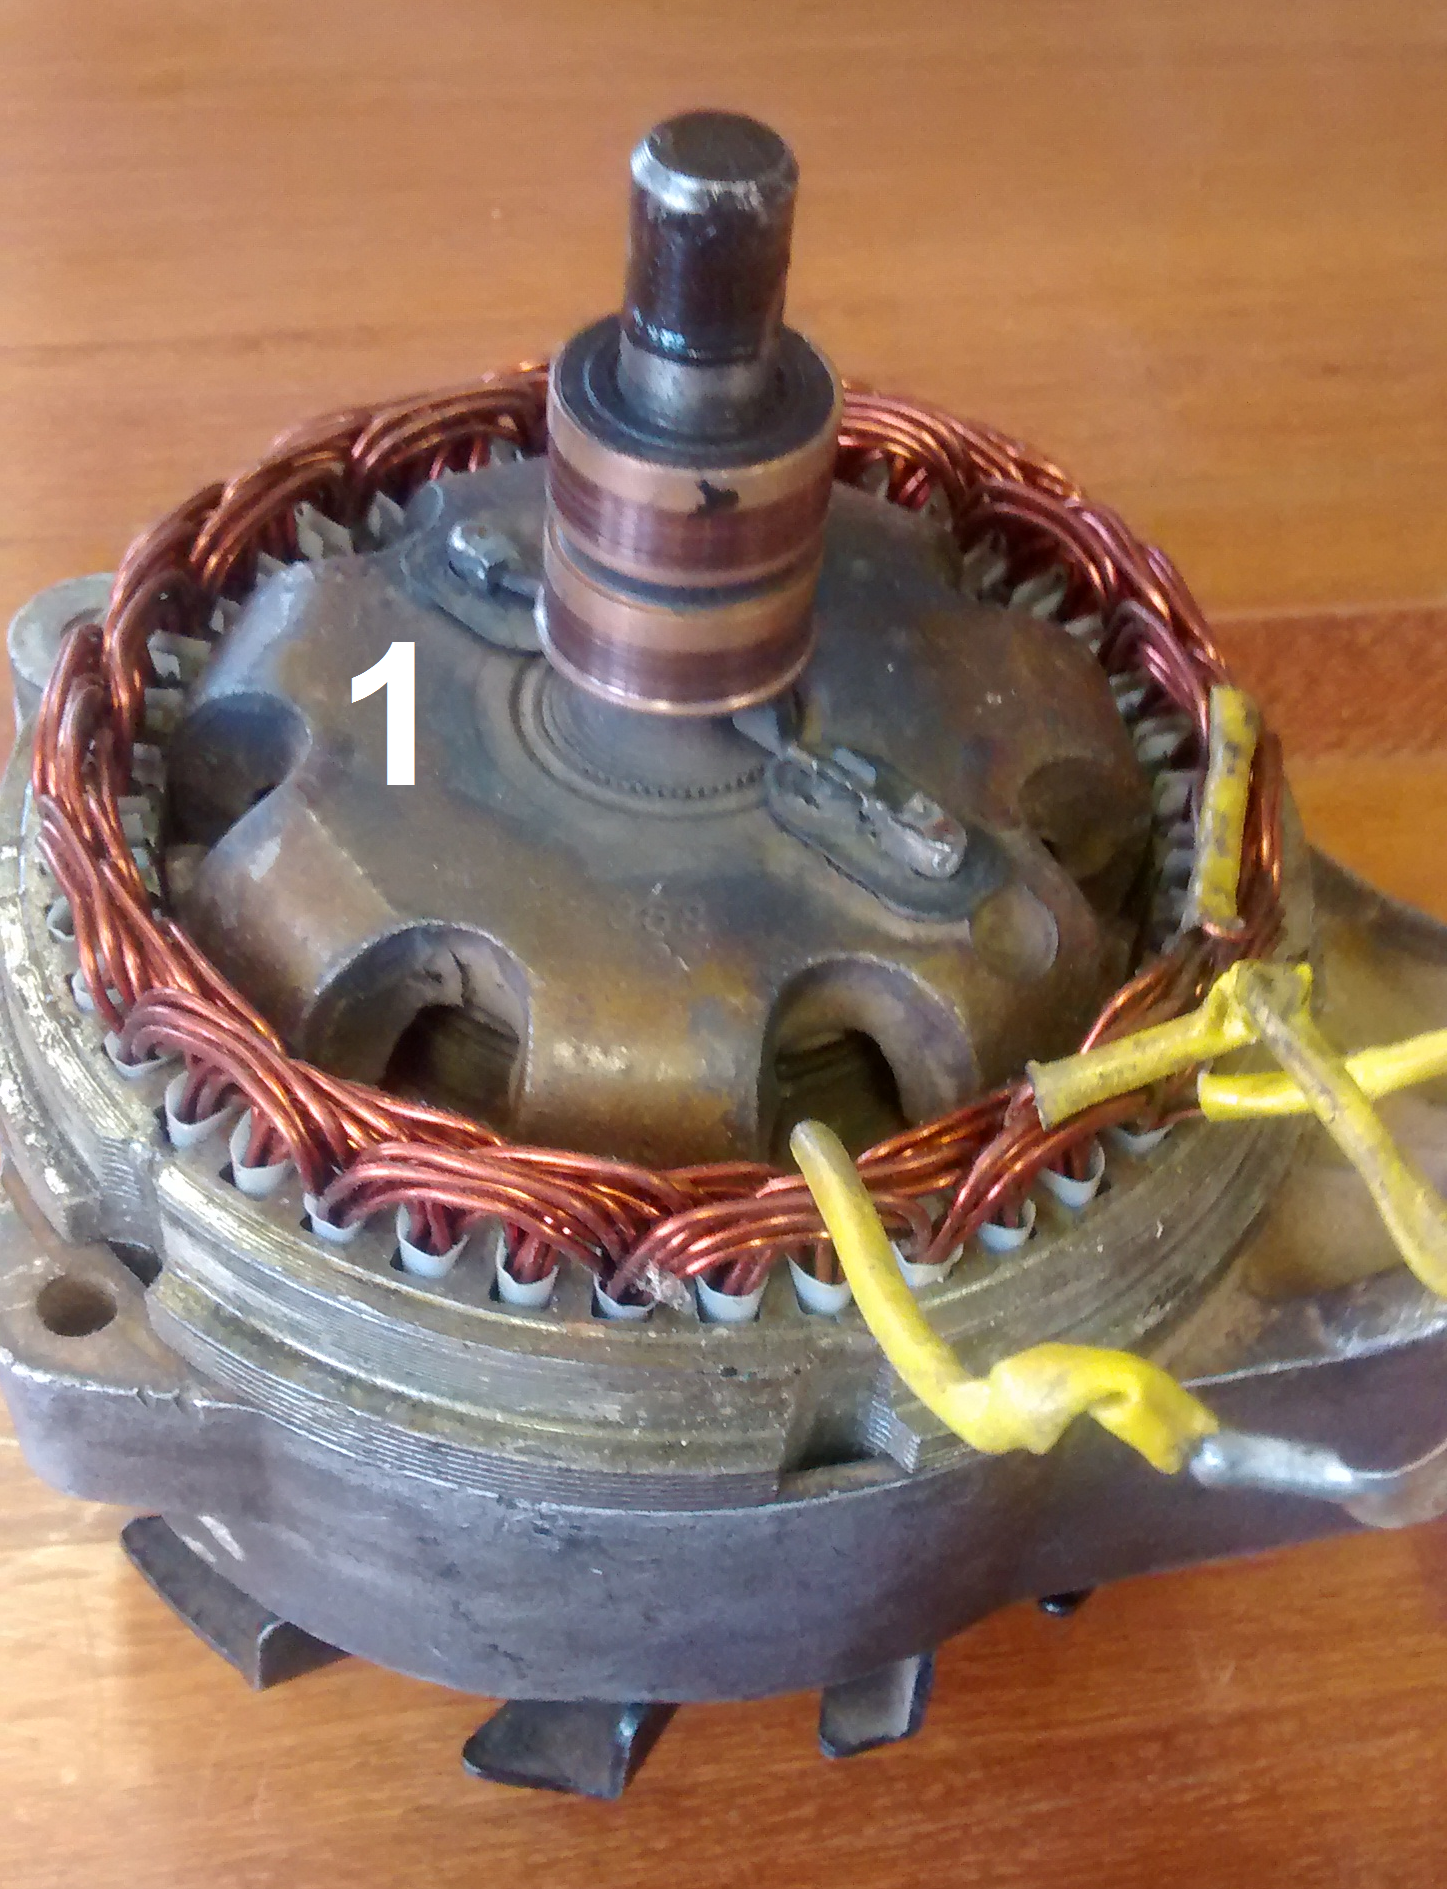
\includegraphics[scale=0.8] {figuras/rotor_alternador.png}
	\caption{Rotor do alternador}
	\label{rotor-alternador}
\end{figure}

\item [Estator]

O estator é formado por um conjunto de bobinas isoladas entre si e fixadas em um conjunto de laminas de aço. Essas lâminas têm características magnéticas de alta permeabilidade, proporcionando um caminho com pequena relutância para o fluxo, o que diminui o fluxo disperso e concentra o campo no entreferro. O uso de lâminas na construção do estator proporciona a diminuição das perdas provocadas por correntes parasitas em relação ao emprego de uma estrutura maciça. Essas lâminas também são tratas termicamente para diminuir o valor das perdas geradas por correntes induzidas.
Essa parte fundamental de um gerador síncrono tem como principal função a criação da corrente elétrica. Entretanto, para a geração de energia as boninas do estator requerem a produção de um campo magnético pelo rotor. A figura \ref{estator-alternador} apresenta o estator do alternador automotivo. 

\begin{figure}[h]
	\centering
	\includegraphics[scale=1]		{figuras/estator_alternador.png}
	\caption{Estator do alternador}
	\label{estator-alternador}
\end{figure}


\item [Regulador de Tensão]

O regulador de tensão do alternador é um dispositivo de proteção do mesmo, utilizado com o objetivo de proteger os equipamentos que usam a energia gerada pelo alternador, ou seja, as cargas conectadas a ele. O regulador protege as cargas por meio do controle da tensão produzida em qualquer regime de rotação do alternador, de modo a limitar a tensão para que não haja picos de corrente elétrica. Além disso, o regulador de tensão é usado com o objetivo de impedir que a bateria utilizada no projeto sofra sobrecarga. 

\item [Ponte Retificadora]
\end{description}

\subsubsection{Alternador Utilizado}

O gerador síncrono utilizado neste projeto trata-se de um alternador do automóvel Chevette com corrente nominal de 35 ampères e tensão de 14 volts. A figura \ref{alternador} apresentada abaixo mostra esse alternador.

\begin{figure}[h]
	\centering
	\includegraphics[scale=0.8]		{figuras/alternador.png}
	\caption{Alternador Utilizado}
	\label{alternador}
\end{figure}

\subsection{Cálculo da Corrente de Projeto Necessária}

A corrente de projeto necessária ao atendimento das cargas a ser alimentadas pelo circuito de distribuição da energia elétrica gerada deve ser determinada conforme a equação abaixo:

\begin{equation}
	\mathcal{I}_{proj} = \frac{{P}_{ativa}}{V \times FP}
\end{equation}

Onde:
\begin{description}

\item [Iproj] corrente de projeto em ampère

\item [Pativa] potência ativa total do circuito em watt

\item [V] tensão do circuito em volt

\item [FP] fator de potência total do circuito
\end{description}

Nesse sentido, com base nos dados informados na Tabela xx da seção xx deste relatório, tem-se que a corrente de projeto será igual a xx A.

	Entretanto, a corrente de projeto a ser adotada para o dimensionamento do circuito elétrico será tida como 35 ampères, devido ao fato deste valor ser a capacidade máxima de corrente elétrica que a fonte geradora aqui adotada poderá atingir.
	
	O fato de a corrente de projeto ter sido escolhida acima da necessidade real de nosso projeto é justificado pelo motivo da possibilidade futura de expansão das cargas alimentadas pelo circuito ora projetado, ocorrendo assim a desnecessidade de redimensionamento do sistema elétrico caso novas cargas fossem inseridas no mesmo.

\subsection{Dimensionamento dos Condutores}

O caminho percorrido pela energia elétrica ao longo de um circuito de distribuição deve ser projetado da maneira mais eficiente possível, desde a fonte geradora de corrente elétrica até as cargas terminais, uma vez que parcela daquela energia é dissipada sob a forma térmica devido à resistência elétrica que o fio condutor pelo qual a referida energia se movimenta exerce sobre o fluxo elétrico, restando, assim, prejudicada a eficiência final de distribuição da energia.

Nesse sentido, ao se projetar um circuito elétrico, deve-se procurar minimizar ao máximo possível as perdas de energia ao longo do mesmo e, agindo dessa maneira, terão sido, por consequência, observados aspectos ambientais e conservacionistas ligados ao desperdício de energia. Ademais, deve-se atentar que as perdas oriundas do calor gerado nos condutores de eletricidade reduzirão o nível da tensão disponível no circuito terminal.

Por isso, ao dimensionar os condutores pertinentes ao projeto elétrico ora em estudo, os aspectos acima mencionados foram levados em consideração, a fim de reduzir na prática as supracitadas perdas.
Seguindo esse raciocínio, a escolha dos condutores utilizados neste projeto foi realizada conforme especificações dispostas pela Associação Brasileira de Normas Técnicas (ABNT) na Norma Brasileira número 5410, de 2004 (NBR 5410:2004), cujo teor aborda critérios para o dimensionamento de instalações elétricas de baixa tensão. 
Desse modo, cuidou-se em dimensionar os referidos condutores de acordo com os critérios que visam auxiliar economia de energia, bem como economia de custos financeiros, a fim de atender às necessidades do nosso projeto.

Assim, conforme especificações técnicas daquela NBR, cuidou-se em identificar a "sessão do condutor que reduza o custo da energia desperdiçada, sem incorrer em custos iniciais excessivos de compra e instalação de um cabo", bem como dos dispositivos de proteção necessários, pautando-se pelos seguintes métodos:

\begin{itemize}
	\item Capacidade de condução de corrente
	\item Queda de tensão
	\item Seção mínima
	\item Proteção contra sobrecarga
	\item Proteção contra curto-circuito
	\item Choque elétrico
\end{itemize}

o final dos resultados, em princípio, cada um desses métodos poderá indicar uma seção diferente. Então, segundo a NBR, a seção a ser finalmente adotada consistirá na maior dentre todas as seções obtidas. Vejamos cada um desses métodos.

\subsubsection{Capacidade de Condução de Corrente (artigo 2)}

Segundo (Eletricidade Moderna), o dimensionamento do projeto elétrico seguindo todos os seis critérios mencionados na NBR em comento, têm sua relevância, embora seja compreensível que o critério da capacidade de condução de corrente apresente uma importância que parece ser superior às demais, surgindo como ponto de partida da escolha dos condutores apropriados.

Ainda no entendimento de (Eletricidade Moderna), o critério aqui discutido, de fato, logo após a determinação das cargas existentes no circuito, passando em seguida pelo cálculo da corrente de projeto ($I_{proj}$), tem como etapa seguinte, sendo considerada a primeira em relação ao dimensionamento dos componentes do circuito, a determinação da capacidade de condução de corrente do circuito, determinando assim a seção do condutor que proporcionará nas condições práticas de execução a capacidade de condução de corrente suficiente para a circulação de $I_{proj}$ sem riscos.

Desse modo, em posse do valor de $I_{proj}$, bem como das características de constituição dos condutores, recorreu-se às tabelas que orientam o dimensionamento através do critério em análise, apurando-se a seção do condutor que atenda às necessidades do nosso circuito, vejamos.

Para o caso concreto,\textit{segundo as disposições da NBR}, quanto ao tipo de condutor empregado, ter-se-á condutor isolado (condutor metálico e isolação), sendo o material PVC (cloreto de polivinila). Isso é devido às características de trabalho listadas na Tabela \ref{nbr}, com informações extraídas da NBR.

\begin{table}[h]
\begin{tabular}{| c | p{3cm} | p{3cm} | p{3cm} |}
\hline
Tipo de isolação                & Temperatura máxima para serviço contínuo (condutor) & Temperatura limite de sobrecarga (condutor) & Temperatura limite de curto-circuito (condutor) \\ \hline
Cloreto de polivinila(PVC)      & 70                                                 & 100                                        & 160                                            \\ \hline
Borracha etileno-propileno(EPR) & 90                                                 & 130                                        & 250                                            \\ \hline
Polietileno-reticulado(XLPE)    & 90                                                 & 130                                        & 250                                           
\\ \hline
\end{tabular}
\caption{Características de condutores. Retirado do}
\label{nbr}
\end{table}

Cumpre informar que o motivo da escolha dos condutores com tipo de isolação PVC foi feita devido esse condutor suportar as condições de nosso projeto.

No que tange ao método de instalação a ser utilizado, levou-se em consideração o fato de que este influencia a capacidade de troca térmica entre os condutores e o ambiente circundante, alterando a capacidade de condução de corrente dos condutores. Por isso, através de visita à Tabela xxxx (abaixo) da NBR, foi definido qual método será o mais adequado às condições de nosso projeto, optando-se pelo método de instalação B1.

\begin{figure}[h]
	\centering
	\includegraphics[scale=0.8]		{figuras/nbr.png}
	\caption{NBR - Definição do método}
	\label{alternador}
\end{figure}

Continuando, a NBR diz que a $I_{proj}$ adotada deve ser corrigida por fatores de correção apropriados, os quais são: a) fatores de correção para temperaturas ambientes diferentes; b) correção de resistividade do solo; e c) fator de correção de agrupamento.

Uma vez que as condições de projeto do circuito em discussão não necessitam da utilização desses fatores, seguiu-se o dimensionamento com a $I_{proj}$ anteriormente informada.

	O próximo passo foi determinar o esquema dos condutores, conforme opções listadas na Tabela \ref{metodo-definicao}. Optou-se pelo esquema monofásico a dois condutores.
	
\begin{table}[h]
\centering
\begin{tabular}{| l | p{7cm} |}
\hline
Esquema de condutores vivos do circuito & Número de condutores carregados a ser adotado \\ \hline
Monofásico a dois condutores            & 2                                             \\ \hline
Monofásico a três condutores            & 2                                             \\ \hline
Duas fases sem neutro                   & 2                                             \\ \hline
Duas fases com neutro                   & 3                                             \\ \hline
Trifásico sem neutro                    & 3                                             \\ \hline
Trifásico com neutro                    & 3 ou 4
\\ \hline
\end{tabular}
\caption{Opções de esquema dos condutores}
\label{metodo-definicao}
\end{table}

Após a definição dessas características/parâmetros, o próximo passo foi consultar a Tabela xxx da NBR para efetivar a escolha da seção dos condutores apropriados às condições de projeto, consoante o critério aqui descrito. Portanto, chegou-se à escolha do condutor de seção xxx.

\subsubsection{Queda de Tensão (disposições da UFJF)}

A importância da aplicação desse critério consiste no fato de que as cargas consumidoras de energia elétrica foram projetadas para trabalharem com determinado valor de tensão, aceitando, apenas, reduzida tolerância de não-conformidade com o valor de tensão nominal para o qual a carga foi projetada.
Assim, ao utilizar esse critério, foi levada em consideração a possibilidade dos efeitos anormais que a queda de tensão poderá acarretar às cargas.
 Segundo esse critério, "à medida que a distância entre o medidor de energia e a potência da carga aumenta a queda de tensão ao longo do condutor também aumenta". 
Por isso, baseando-se nesse critério, e com auxílio das características dos condutores adotados neste projeto (PVC, eletroduto não magnético e método de referência B1), somado ao fato de que a NBR informa que em baixa tensão, a queda de tensão nos circuitos terminais não pode ser superior a 4\%, calculou-se a seção dos condutores, veja.

\begin{description}

	\item Cálculo da Queda de Tensão
	%pegar as equaçoes
	
	Com esse resultado, visitou-se a Tabela xxx da fabricante \textit{Pirelli} e constatou-se que para as condições do nosso projeto, a seção do condutor deve ser 6 mm\textsuperscript{2}.
(Lembrar que deve ser atentado ao cálculo da queda de tensão por trecho)

\begin{equation}
	\Delta V = \Delta V_{\frac{V}{A \times km}} \times I_{proj} \times L
\end{equation}
\begin{equation}
	\Delta V_{\frac{V}{A \times km}} = \frac{\Delta V} {I_{proj} \times L}
\end{equation}
\begin{equation}
	\Delta V_{\frac{V}{A \times km}} = \frac{0,04 \times 14}{35 \times 0,002}
\end{equation}
\begin{equation}
	\Delta V_{\frac{V}{A \times km}} = 8 \times \frac{V}{A \times km}
\end{equation}

\end{description}

\subsubsection{Seção Mínima}

As seções mínimas admitidas em qualquer instalação de baixa instalação estão indicadas na Tabela \ref{secoes-minimas}, item xxx da referida Norma. Nesse quesito, traduz-se a tabela, abaixo:

\begin{table}[h]
\begin{tabular}{ |l | p{7cm} | p{5cm} |}
\hline
Instalação                          & Número de condutores carregados a ser adotado           & Seção Mínima para condutores de cobre (mm\textsuperscript{2}) \\ \hline
\multirow{3}{*}{Fixas em geral}     & Circuitos de Iluminação                                 & 1,5                                        \\ \cline{2-3}
                                    & Circuitos de Força                                      & 2,5                                        \\ \cline{2-3}
                                    & Circuitos de sinalização e controle                     & 0,5                                        \\ \hline
\multirow{3}{*}{Ligações flexíveis} & Para um equipamento específico                          & Como especificado na norma do equipamento  \\ \cline{2-3}
                                    & Para qualquer outra aplicação                           & 0,75                                       \\ \cline{2-3} 
                                    & Circuitos a extrabaixa tensão para aplicaçòes especiais &                                           
\\ \hline

\end{tabular}
\caption{Seções Mínimas}
\label{secoes-minimas}
\end{table}

Assim, dentro desse quesito, adotou-se que as ligações de nosso circuito serão do tipo flexíveis, sendo a utilização consistente com circuitos de extra-baixa tensão para aplicações especiais. 

Por isso, levando-se em consideração a Tabela \ref{secoes-minimas}, a seção indicada é 0,75 mm\textsuperscript{2} para os condutores de cobre.

\subsubsection{Outros}

Porém, "como isto significa aumentar o custo do cabo, tende-se a anular a economia conseguida pela melhoria da eficiência na distribuição, sendo que é necessário encontrar-se então um compromisso entre estas duas variáveis".

Por isso, visando economia de energia e uma distribuição de alta eficiência, procurou-se escolher os condutores deste projeto portando-se pela NBR em comento.

\subsection{Dimensionamento dos Dispositivos de Proteção do Circuito}

A proteção é uma ação automática provocada por dispositivos sensíveis a determinadas condições anormais, no sentido de evitar ou limitar danos a um sistema ou equipamento, a proteção também pode ser entendida como uma manobra automática.

A escolha, aplicação e a coordenação seletiva adequadas ao conjunto de componentes que constituem a proteção de um sistema é um dos aspectos mais importantes da instalação elétrica industrial. A função da proteção justamente minimizar os danos ao sistema e seus componentes, sempre que ocorrer uma falha no equipamento, no sistema elétrico ou falha humana.

Os dispositivos de proteção contra correntes de curto-circuito, como: disjuntores e fusíveis. E os dispositivos de proteção contra correntes de sobrecarga, como os relés bimetálicos.
\part{Resultados e Conclusões}
\chapter[Resultados]{Resultados}

Com a inclusão dos sensores no sistema, espera-se coletar dados que são considerados importantes para as mudanças físicas que irão ocorrer no ambiente virtual, bem como causar sensações no usuário de forma que o mesmo tenha um experiência semelhante a andar de bicicleta na rua. Os seguintes dados serão coletados: velocidade, direção a qual o guidão é movimentado e nível da bateria para o sistema de realimentação.

Os dados da velocidade serão apresentados ao atleta para que ele tenha consciência do seu desempenho. O sinal do sensor de direção do guidão fará com que haja uma alteração no ambiente virtual, ou seja, dependendo da angulação do guidão, o usuário terá a sensação de que está fazendo uma curva. Outro dado importante é que quando houver uma subida no percurso do ambiente virtual o usuário terá maior dificuldade ao pedalar, como se realmente estivesse subindo um morro, por exemplo.

Por meio destas características, espera-se simular um ambiente que seja tão próximo quanto possível da realidade de forma a tornar atividades físicas, como o \textit{spinning}, algo menos monótono já que o atleta não se desloca e apresentar dados que possam melhorar seu rendimento. Outro resultado interessante é realizar a comparação do nível de iteratividade do sistema com uma situação real e analisar como o usuário se comporta em ambos os ambientes. Isso é interessante para atletas de alto nível pois simular o percurso de uma prova e ter conhecimento das reações do corpo naquele ambiente é de fundamental importância para um bom desempenho.

\chapter{Manual do Produto} % (fold)
\label{cha:manual_do_produto}
 
O trecho a seguir descreve o processo recomendado pela equipe para o uso do produto, assim como os cuidados que devem ser tomados com o manuseio.

\section{Modo de Uso} % (fold)
\label{sec:modo_de_uso}

\begin{enumerate}
	\item Verifique se a aplicação já esta em funcionamento com o auxilio da tela secundaria (notebook/monitor).
	\item Posicione-se sobre a bicicleta. Verifique se a mesma se mantem  estável com o seu peso. Para mais informações sobre os valores para qual este produto foi projetado, verificar \autoref{dados-usuario}.
	\item Imerja-se na realidade virtual com o \gls{rift}.
	\item Após o uso do equipamento, remova o \gls{rift} e espere de 15 a 30 segundos antes de tentar desmontar da bicicleta\footnote{Devido a alta imersão, é recomendado um tempo para se acostumar novamente com a realidade antes de realizar movimentos bruscos.}.
\end{enumerate}

\section{Precauções} % (fold)
\label{sec:precau_es}

\begin{description}
	\item [Não tente desmontar da bicicleta utilizando o gls{rift}] $-$ Ao utilizar o \gls{rift}, a imersão proporcionará uma perca da noção de espaço e posição da realidade. Tentar se movimentar na realidade visualizando o ambiente virtual é extremamente desencorajador.
	\item [Não grite] $-$ A imersão no ambiente virtual causa uma perca de contato com a realidade, lembre-se disto antes de tentar se comunicar com aqueles que te assistem.
	\item [Evite balançar muito na bicicleta ou ficar em pé nela] $-$ Apesar de cálculos terem sido feitos no intuito de manter a bicicleta o mais estável possível ao chão, o produto ainda é passível de tombamento quando exposto a determinados momentos angulares.
	\item [Divirta-se] $-$ Mesmo tendo como objetivo apresentar uma alternativa para a pratica de atividades físicas em ambientes fechados, o projeto busca oferecer também entretenimento ao usuário.
	\item [Mantenha o produto] $-$ Evite reajustar os sensores, a altura do guidão ou do banco. Por ser um protótipo, o produto ainda não oferece um amplo grau de personalização. Tentar configurar o equipamento sem o devido conhecimento do produto pode vir a danifica-lo ou  ao comprometimento dos sinais adquiridos para controle do ambiente.
\end{description}

\begin{anexosenv}


\chapter{Entrevista por Pauta}

\textbf{Entrevistado:} Leandro Luiz Fleury Rosa

\textbf{Profissão:} Optometrista

\textbf{Local:} Ótica Cristal (Goiânia)

\textbf{Pauta:}

\begin{enumerate}
\item Como surgiu a ideia ou a necessidade de um produto como esse?
\item Qual a faixa etária mais comum dos usuários de lente e possíveis usuários do produto?
\item Pela sua experiência, é grande a quantidade de pessoas que tem dificuldade de utilizar lentes? Quais pessoas possuem mais dificuldade?
\item Quais as principais características de uma lente rígida (gás permeável) e de uma lente gelatinosa? Diâmetro, textura, maliabilidade, resistência e etc.
\item Como é feita higienização ou limpeza da lente?
\item Como um dos mentores da ideia, quais as principais funcionalidades que você acredita que produto deve ter? Quais os principais benefícios?
\item Qual a sua opião sobre um processo de limpeza da lente ser integrado ao produto?
\item Existe algo que contém caracteristicas similares a um olho humano a fim de realizar testes do aparelho?
\item Explicar conceito inicial desenvolvido pela equipe para o produto e coletar opinião. 
\item Verificar possibilidade de doação de materiais.
\end{enumerate}


\chapter{Fundamentação Teórica}

\section[Instrumentação e Sensoriamento]{Instrumentação e Sensoriamento}

\subsection[Processamento de Imagens]{Processamento de Imagens}

Processamento de imagens consiste de qualquer forma de processamento de dados no qual a entrada e saída são imagens, tais como fotografia ou quadros (\textit{frames}) de algum vídeo. Geralmente esta técnica é utilizada para aprendizado de máquina ou detecção de padrões, sendo que a segunda, para este trabalho, é a mais relevante.

Na literatura consultada, são apresentadas várias técnicas de detecção de padrões com o objetivo de detectar a face e o olho em uma imagem. \citeonline{hsu} apresenta um método de detecção para ambientes onde a luz varia bastante ao longo do dia, dessa maneira o método consiste primeiramente de procurar candidatos baseando-se na cor da pele, e então através de uma análise de crominâncias, encontra-se possíveis regiões para olho, boca e nariz. 

\citeonline{huang} propuseram uma combinação de abordagens para solucionar o problema da detecção robusta de faces e olhos. Em imagens de faces de baixa resolução, os olhos e as sobrancelhas se apresentam como barras escuras que podem ser detectadas utilizando a segunda derivada de um filtro Gaussiano. Por isso aplicaram filtros Gaussianos e direcionais para detectar candidatos a olhos, sobrancelhas, boca e nariz. Após este passo, um modelo estrutural é criado para agrupar pontos característicos de candidatos à face usando relações geométricas.

Um dos algoritmos mais eficazes para a detecção de faces e olho em imagens estáticas é o algoritmo de \citeonline{viola}, que se encontra implementado na biblioteca Intel OpenCV (Intel Open Source Computer Library) e que visa localizar em uma imagem características que codifiquem alguma informação do padrão sendo detectado. Esses padrões são baseados nas características de Haar que codificam informações sobre a existência de contrastes orientados entre regiões da imagem. A Figura \ref{fig09} apresenta algumas características de Háar propostas para a detecção de faces em imagens estáticas.  


\begin{figure}[htb]
		\centering
			\includegraphics[scale=0.7]{figuras/haar.png}
		\caption{Características de Haar mais usadas em detecção de faces}
		\label{fig09}
\end{figure}

Quando as características de Haar são aplicadas em uma imagem, são examinados os contrastes naturais proporcionados pelas características da face, considerando suas relações de espaço, como ilustrado na Figura \ref{fig10}.


\begin{figure}[htb]
		\centering
			\includegraphics[scale=0.7]{figuras/haar2.png}
		\caption{Relação entre as características de Haar e os contrastes naturais da face}
		\label{fig10}
\end{figure}

De forma a complementar a detecção de possíveis regiões dos olhos através do algoritmo de Viola-Jones, é possível usar a técnica apresentada por \citeonline{hsu}, onde diz que para uma imagem no espaço de cores YCbCr, os olhos apresentam um alto valor de Cb e baixo valor para Cr. Dessa forma, ele apresenta um conjunto de operações entre o plano Cb e Cr com o objetivo de isolar as possíveis regiões de olho.

\subsection[Sensor de Proximidade Ultrassônico]{Sensor de Proximidade Ultrassônico}

Um sensor de proximidade ultrassônico possui uma alta aplicabilidade em pesquisas e indústrias. Essa alta aplicação dá-se devido a sua detecção de objetos de texturas, formas, cores e materiais diferentes, sendo assim aplicável para detecção de distancia, altura, medida de diâmetro, contagem de objetos entre outras.

Com o funcionamento baseado na emissão de ondas sonoras de alta frequência, o sensor de proximidade ultrassônico funciona medindo o tempo entre a emissão e a recepção da onda gerada pelo sensor. Esta onda, ao sair do sensor, bate no objeto que está mais próximo gerando um eco, que por sua ver volta para o sensor que é capaz de calcular a distância entre o emissor e objeto sabendo a velocidade da onda emitida e o tempo que essa onda levou para chegar novamente ao receptor, gerando assim um sinal elétrico proporcional.

\begin{figure}[htb]
		\centering
		\includegraphics[scale=0.7]{figuras/sensorultra.png}
		\caption{Sensor de Proximidade Ultrassônico}
		\label{fig11}
\end{figure}

Como o espalhamento das frentes de onda destes sensores têm forma cônica, eles podem ser ajustados de maneira que o cone alcance maior distância e precisão para detecção de um determinado objeto (Fig. \ref{fig11}).

A maioria dos sensores comercializados hoje pela indústria eletrônica são capazes de detectar objetos a distancias entre 2 cm a 450 cm com uma precisão de 3 mm. Esses objetos não precisam necessariamente estarem parados na frente do sensor devido a alta velocidade de propagação da onda emitida, sendo o seu uso possível em processos de fabricação contínuos que utilizam esteiras.
 
\subsection[Sensor de Toque]{Sensores de Toque}

Sensores de toque são basicamente transdutores com sensibilidade para força, pressão ou toque humano. Esses tipos de sensores são bastante utilizados nos dias atuais, visto que os mesmos estão presentes em aplicações do tipo \textit{touch screen}, muito comum em \textit{tablets}, \textit{smartphones}, agências bancárias, \textit{notebooks}, etc.

O primeiro sensor de toque foi desenvolvido em 1971 pelo fundador da Elographics Dr. Sam Hurst e, ainda durante a década de 90, teve sua adoção disseminada com a criação dos \textit{smartphones} e demais equipamentos que utilizam a tecnologia \textit{touch screen}, como ATMs e sistemas de pontos de vendas. O uso da tecnologias \textit{touch} disseminou rapidamente quando o iPhone introduziu as habilidades de múltiplos toques e zoom utilizando estes tipos de sensores \cite{mathas}.

Os principais tipos existentes de sensores de toques são os resistivos, capacitivos, infravermelhos, e de superfície acústica (SAW, do inglês \textit{Surface Acoustic Wave}). Cada um deles podendo detectar o toque de uma forma diferente e, em alguns casos, podendo detectar gestos sem contato direto \cite{mathas}.

No presente projeto, o estudo dos sensores de toque será focado para avaliar se este tipo de sensor é apropriado para fornecer uma medida altamente precisa do momento em que a ventosa, com ou sem a lente, encosta no globo ocular do usuário da máquina. 

Devido a característica do projeto, as habilidades de zoom ou múltiplos toques que podem ser obtidos com esses sensores são irrelevantes. Apenas é necessário apontar características como sensibilidade, precisão, robustez, tamanho e custo, para saber se a medida é confiável para controlar a proximidade e toque com o olho, se o sensor é pequeno e robusto o suficiente para não apresentar falhas e ser fácil de integrar com o projeto mecânico do protótipo e se o mesmo possui custo baixo visando tornar o preço do produto final e do protótipo mais acessível. Sendo assim, as características que serão apresentadas abaixo abordarão os requisitos supracitados.

\subsubsection[Princípios de Funcionamento]{Princípios de Funcionamento}

Antes de focar nas características listadas anteriormente, é válido conhecer o princípio de funcionamento dos mesmos, de modo a restringir a pesquisa futura somente nos que realmente sejam relevantes para o projeto.



Os sensores de toque capacitivo são baseados em perturbações elétricas. Os sensores deste tipo são constituídos por lâminas de vidros que possuem um revestimento condutor de um lado e um padrão de circuito impresso ao redor da área de visualização. Basicamente, o padrão de circuito impresso cria uma carga em toda superfície do sensor, que é perturbada quando se toca com o dedo, luva ou qualquer outro objeto na tela do sensor \cite{mathas}. Conforme pode ser visualizado na Fig. \ref{fig12}.

O dedo ou qualquer outro objeto aterrado serve como uma fonte de excitação que, quando encostado na superfície metálica da lâmina de vidro, gera uma perturbação no campo elétrico que será transmitido para o padrão de circuito impresso. Tal perturbação passa por um conversor ADC (\textit{Analog to Digital Converter}) para ser, posteriormente, tratada no domínio digital \cite{ad7142} como mostra a Figura \ref{fig12}.

A interferência no campo elétrico induzido é gerada pelo desvio de linhas de campo elétrico que são desviadas para a terra e não atingem o receptor. Desta forma, ocorre uma diminuição da capacitância total medida pelo receptor\cite{ad7142} de acordo com a lei da capacitância:

$$ C = \frac{Q}{V} $$

Por serem construídos sobre o vidro, não é necessário muita pressão para obter resposta desse tipo de sensor de forma que a força é insignificante. A única desvantagem é que esses sensores são vulneráveis à abrasão do revestimento condutor \cite{mathas}.

De todos os tipos de sensores de toque este é o único que permite a tecnologia de múltiplos toques e, por isso, é muito utilizado em \textit{smartphones}, porém a utilização deste tipo de sensor tem aumentado em para aplicações industriais, médicas, automotivas e de consumo \cite{mathas}. 

\begin{figure}[htb]
		\centering
			\includegraphics[scale=0.7]{figuras/sensortoque.png}
		\caption{Sensor de Toque}
		\label{fig12}
\end{figure}




O sensor de toque resistivo consiste em duas camadas que não estão em contato e separadas por um espaço bem fino. Quando ocorre uma pressão causada pelo toque, essas camadas se tocam modificando a resistência do conjunto e causando uma resposta do sensor, confirma mostra a Figura \ref{fig13} \cite{keyur}.

\begin{figure}[htb]
		\centering
			\includegraphics[scale=0.7]{figuras/variacao.png}
		\caption{Variação de Resistência}
		\label{fig13}
\end{figure}

Este tipo de sensor é a forma mais comum de sensores de toque existentes sendo usados para aplicações de distância e pressão. Em geral, este tipo de sensor é mais simples e barato. Suas limitações consistem em uma falha ocasionada pela falta de flexão necessária para empurrar o conjunto de superfícies, a redução do brilho que atravessa este sensor (queda de 10\% a 20\%) e o fato de não suportar múltiplos toques \cite{mathas}.

Este tipo de sensor oferece um custo benefício bom, leituras consistentes, desempenho durável em ambientes onde é necessário suportar contaminantes e líquidos tais como restaurantes fábricas e hospitais. Estes sensores, em geral, são muito utilizados em \textit{gadgets} e aplicações de consumo portátil \cite{mathas}.



Já os sensores de toque infravermelho trabalham com uma face de vidro em frente do LCD. Existem emissores de luz infravermelha e sensores nas quatro direções de observação, onde esses emissores ficam constantemente enviando feixes de luz infravermelha. Quando ocorre o toque, os feixes de luz são interrompidos ou alterados, o que é perceptível pelos sensores, conforme mostra a Figura \ref{fig14} \cite{vicki}. Dessa forma a pressão do toque e o objeto utilizado para efetuar o toque são irrelevantes, este tipo de sensor é mais comum de ser utilizado em aplicações envolvendo jogos e quiosques de informação \cite{mathas}.


\begin{figure}[htb]
		\centering
			\includegraphics[scale=0.7]{figuras/infra.png}
		\caption{Sensor de Toque Infravermelho}
		\label{fig14}
\end{figure}



O funcionamento do sensor SAW, por sua vez é bastante similar ao dos sensores de toque infravermelho. A diferença consiste que, em vez de feixes de luz, serão emitidos impulsos ultrassônicos gerados por cristais piezelétricos. Estes cristais são ligados no vidro da superfície para criar os impulsos de som que se deslocam ao longo da superfície. Nesta configuração, é necessária a presença de refletores que redirecionam o som de volta aos cristais que, por sua vez, convertem as ondas mecânicas em energia elétrica \cite{mathas}.  

Quando ocorre um toque, parte do som é absorvida ou redirecionada, e assim é possível através de alguns sensores, calcular a posição onde se foi realizado o toque. Em geral esse tipo de sensor é utilizado em caixas eletrônicos, quiosques de informação e parques de diversões \cite{mathas}.

Através do principio de funcionamento dos sensores mencionados acima, é possível verificar que os sensores de toque infravermelho e SAW são mais apropriados para aplicações que envolvam uma interação com usuário através da tecnologia \textit{touch screen}. Para o sensoriamento que se deseja neste projeto, a utilização de sensores de toque capacitivos ou resistivos se torna mais adequada.

Desta forma foi levantado alguns modelos comerciais destes dois tipos de sensores visando principalmente verificar características como o tamanho do sensor, robustez, precisão, sensibilidade e preço.

\subsubsection[Modelos Comerciais]{Modelos Comerciais}

A Figura \ref{fig15}  relaciona modelos comerciais de sensores de toque capacitivos e resistivos com suas respectivas características. Devido a questões práticas, de aquisição de material, buscaram-se os sensores da marca freescale semiconducter, devido a mesma possuir diversos distribuidores localizados no Brasil.
	
Devido ao principio de funcionamento dos sensores resistivos e capacitivos, eles possuem sempre uma alta sensibilidade ao toque, e uma alta precisão para detectar o momento do toque. Quanto a robustez é válido lembrar que o sensor resistivo pode apresentar falhas referentes a flexão ocasionada pelo toque na lâmina e que o sensor capacitivo pode vir a sofrer abrasão do revestimento condutor. Desta forma será listado alguns modelos, o tipo do modelo, tamanho e custo.

\begin{figure}[htb]
		\centering
			\includegraphics[scale=1.0]{figuras/toquecomerciais.png}
		\caption{Sensores de toques disponíveis no site da freescale semiconducter para venda \cite{free}.}
		\label{fig15}
\end{figure}


\subsection[Sensores de Pressão]{Sensores de Pressão}

Sensores são dispositivos projetados para detectarem algum evento no processo e emitirem um sinal de resposta a esse evento \cite{geomar}. É a parte sensitiva de um transdutor, que é um sistema que transforma duas formas de energia para fins de medida \cite{werneck}.

A pressão é uma força por uma unidade de área que um corpo exerce sobre o outro. As unidades comuns dos sensores de pressão são psi [$lb/pol^2$] e Pa [$N/m^2$]. As medidas de pressão são feitas para gases e líquidos.

A ideia básica para que o dispositivo pegue a lente do seu estojo e a mantenha na ventosa é trabalhar com pressão negativa para sucção da lente. A ventosa citada já é vendida no mercado e funciona justamente para auxiliar pessoas com dificuldade na manipulação de lentes de contato. No contexto deste projeto, vê-se a necessidade de monitorar a pressão no interior da ventosa, para que esta pressão não ultrapasse um limiar ideal de seguridade.

Os valores normais de pressão intraocular estão compreendidos entre 10 e 21 mmHg aproximadamente \cite{andre}. Os sensores serão, então, avaliados principalmente pelo range citado, precisão, sensibilidade, robustez.

\subsubsection[Princípio de Funcionamento]{Princípio de Funcionamento}

Os sensores de pressão são compostos por duas partes: a conversão de pressão em uma força ou deslocamento e conversão de força e deslocamento em sinal elétrico \cite{geomar}.

Os sensores de pressão podem ser classificados em três tipos, de acordo com a referência utilizada para a leitura \cite{patsko}:
\begin{itemize}
\item Sensores de pressão \textit{Gauge}: medem a pressão de interesse em relação à pressão atmosférica local;
\item Sensores de pressão diferencial: medem a diferença de pressão entre dois pontos distintos no circuito, onde nenhum deles está na pressão atmosférica necessariamente. Possui duas entradas de ar e o nível de tensão da saída indica a diferença entre as pressões;
\item Sensores de pressão absoluta: medem a pressão de interesse em relação em relação ao vácuo total (0 psi).
\end{itemize}

Os sensores de pressão são, dentre outros métodos, geralmente construídos com materiais piezoresistivos. Esses materiais possuem a capacidade de variar sua resistência  quando submetidos a um esforço mecânico. São construídas duas câmaras e entre elas é colocada uma película de material piezoresistivo, como ilustrado na figura \ref{fig16}. O modo como essas câmaras são construídas é que define qual é o tipo do sensor. Em um sensor de pressão absoluta, uma dessas câmeras é fechada e outra é aberta, destinada à pressão a ser medida. A câmara fechada contém vácuo, ou seja, a pressão a ser monitorada é medida em relação à pressão zero. Esse sensor é ideal para medir pressões baixas, menores do que a atmosférica \cite{patsko}.

Num sensor \textit{Gauge}, as duas câmaras são abertas, sendo que uma é destinada a pressão a ser medida, enquanto que outra é destinada a entrada de ar atmosférico. Desse modo, a pressão é medida em relação à pressão atmosférica local. Caso a pressão externa seja igual à utilizada como referência para o sensor, a força resultante sobre o material piezoresistivo será nula. Se uma das pressões for maior do que a outra, temos que a película será submetida a um esforço e sua resistência irá mudar. O sensor de pressão diferencial também possui as duas câmaras abertas, porém elas são destinadas às pressões que serão comparadas pelo sensor \cite{patsko}. Os valores comerciais dos sensores piezoresistivos são nas faixas de 0 a 1,5 psi e 0 a 5000 psi \cite{geomar}.

Nos modelos de sensores piezoresistivos, a estrutura é construída utilizando a tecnologia MEMS, que possibilita a sua montagem em dimensões extremamente reduzidas, possibilitando a integração de todos os componentes numa única peça.

\begin{figure}[htb]
		\centering
			\includegraphics[scale=0.7]{figuras/sensorpressao.png}
		\caption{Sensores de pressão a semicondutor \cite{geomar}.}
		\label{fig16}
\end{figure}

O tubo de Bourdon é um medidor de pressão de grande importância no âmbito industrial, sendo uma das soluções mais utilizadas. O funcionamento deste tipo de manômetros é baseado na alteração da curvatura originada num tubo de secção elíptica pela pressão exercida no seu interior. A secção elíptica tende para uma secção circular com o aumento da pressão no interior do tubo levando a que o tubo se desenrole. Este tubo tem a uma das extremidades fechadas e ligada a um mecanismo, com rodas dentadas e mecanismos de alavanca, que permite transformar o seu movimento de "desenrolar", originado pelo aumento de pressão no interior do tubo, no movimento do ponteiro do manômetro \cite{bourdon}. O tubo de Bourdon é disponível para pressões de 30 a 100.000 psi \cite{geomar}.

\begin{figure}[htb]
		\centering
			\includegraphics[scale=0.7]{figuras/bourdon.png}
		\caption{Ilustração do tubo de Bourdon. Um sensor de posição , como um LVDT, transforma o deslocamento em um sinal elétrico \cite{geomar}.}
		\label{fig17}
\end{figure}

\subsubsection[Modelos comerciais]{Modelos comerciais}

São apresentados  na figura \ref{fig18} alguns modelos comerciais de sensores de pressão que podem ser utilizados na prototipação do projeto. Como a pressão do olho é de 10 a 21mmHg, 1,3Kpa a 2,8KPa os sensores cabíveis são os com princípio piezoresistivo.

\begin{figure}[htb]
		\centering
			\includegraphics[scale=0.8]{figuras/pressaocomerciais.png}
		\caption{Modelos comerciais de sensores cabíveis ao projeto \cite{free2}.}
		\label{fig18}
\end{figure}







\section[Controle e Atuação]{Controle e Atuação}

\subsection[Atuadores]{Atuadores}

Em um sistema, atuador é um elemento que atende a comandos do controlador e produz movimento. Em linhas gerais, o atuador transforma algum tipo de energia de entrada em movimentos, que pode ser considerado energia cinética. Os atuadores podem ter seu movimento induzido por força de origem pneumática, hidráulica, elétrica, combustão ou até mesmo por deformação termal de materiais \cite{machado}.

Ainda, os atuadores podem fornecer basicamente dois tipo de movimento: 1) rotativo: como é o caso dos motores e; 2) linear (ou translação): como é o caso dos pistões e solenoides que podem oferecer um avanço ou recuo. A escolha do atuador deve ser feita a partir deste requisito inicial, contudo, é possível converter um tipo de movimento no outro. Para converter um movimento rotativo em linear, pode-se utilizar um sistema de pinhão e cremalheira ou eixo acoplado a rosca sem fim. Para converter um movimento linear em rotativo, pode-se utilizar o sistema de biela e eixo assimétrico, como o existente nos motores dos veículos \cite{machado}.

Os atuadores rotativos ainda podem ser classificados em:
\begin{itemize}
	\item angulares: quando giram apenas num ângulo limitado, como é o caso dos servomotores e motores de passo;
	\item contínuos: que têm a possibilidade de realizar número indeterminado de rotações, como é o caso dos motores de corrente contínua.
\end{itemize}

Tal como o nome sugere, um servomecanismo deve obedecer a comandos. Sendo este geralmente interligado a um sistema de malha fechada com realimentação, ele informa ao controlador se a tarefa foi executada. O controlador monitora a atuação do servomecanismo e através de sensores de posição e compensa eventuais discrepâncias entre o valor desejado e o valor obtido \cite{SCME}.



\subsubsection[Tipos de Atuadores]{Tipos de Atuadores}

Será feita adiante uma breve explicação sobre cada tipo de atuador existente, explicitando suas características genéricas e pontuando quais tipos são mais adequados para este projeto.

\textbf{Motores Elétricos de Corrente Contínua (CC)}

Os motores elétricos são máquinas elétricas que caracterizam atuadores do tipo rotativo e podem ser subdivididos em motores angulares ou de rotação contínua. 

Em se tratando de aspectos construtivos, o motor CC pé composto por duas estruturas magnéticas \cite{siemens}:
\begin{itemize}
	\item Estator (enrolamento de campo ou imã permanente)
	\item Rotor (enrolamento de armadura)
\end{itemize}

O estator é composto de um imã permanente ou de uma estrutura ferromagnética onde são enroladas bobinas que formam o campo. Já o rotor é um eletroímã  constituído de um núcleo de ferro com enrolamentos em sua superfície que são alimentados por um sistema mecânico de comutação como mostra a Figura \ref{estruturamotor}.

\begin{figure}[htb]
		\centering
			\includegraphics[scale=0.9]{figuras/estruturamotorcc.png}
		\caption{Estrutura de um motor CC \cite{siemens}}
		\label{estruturamotor}
\end{figure}

Quanto ao seu tipo de configuração de enrolamentos, podem ser classificados de acordo com o organograma da Figura \ref{fig19} \cite{siteeducation}:

\begin{figure}[htb]
		\centering
			\includegraphics[scale=0.9]{figuras/motores1.png}
		\caption{Classificação dos motores quanto ao tipo \cite{siteeducation}}
		\label{fig19}
\end{figure}

Os motores de corrente alternada (CA) não aparecem na figura acima, pois não são recomendados para aplicações de baixa potência onde prevalece o controle de pequenos sinais elétricos. Dependendo da aplicação, os acionamentos em corrente contínua são geralmente os que apresentam os maiores benefícios, também em termos de confiabilidade, operação amigável e dinâmica de controle. Assim, podemos enumerar algumas vantagens \cite{siemens}:
\begin{itemize}
	\item Operação em 4 quadrantes com custos relativamente mais baixos; 
	\item Ciclo contínuo mesmo em baixas rotações;
	\item Alto torque na partida e em baixas rotações;
	\item Ampla variação de velocidade;
	\item Facilidade em controlar a velocidade;
	\item Os conversores CA/CC requerem menos espaço;
	\item Confiabilidade;
	\item Flexibilidade (vários tipos de excitação);
	\item Relativa simplicidade dos modernos conversores CA/CC.
\end{itemize}

E desvantagens:
\begin{itemize}
	\item Os motores de corrente contínua são maiores e mais caros que os motores de indução, para uma mesma potência;
	\item Maior necessidade de manutenção (devido aos comutadores);
	\item Arcos e faíscas devido à comutação de corrente por elemento mecânico (não pode ser aplicado em ambientes perigosos);
	\item Tensão entre lâminas não pode exceder 20V, ou seja, não podem ser alimentados com tensão superior a 900V, enquanto que motores de corrente alternada podem ter milhares de volts aplicados aos seus terminais;
	\item Necessidade de medidas especiais de partida, mesmo em máquinas pequenas (uso de \textit{soft starters}.
\end{itemize}

A classificação dos motores de corrente contínua é dada de acordo com o tipo de excitação de seus enrolamentos do campo e da armadura. A Figura \ref{fig20} mostra a configuração dos enrolamentos de cada tipo de motor CC \cite{siteeducation}.

\begin{figure}[htb]
		\centering
			\includegraphics[scale=0.9]{figuras/motores2.png}
		\caption{Tipos de motores de corrente contínua: a) motor de imã permanente; b) motor de excitação separada; c) motor de excitação série; d) motor de excitação shunt; e) motor de excitação mista \cite{siteeducation}}
		\label{fig20}
\end{figure}

Cada tipo de configuração apresenta características diferentes de acordo com o que se segue \cite{siemens}:

\par \vspace{\baselineskip}
\par \vspace{\baselineskip}

\noindent
Motor de excitação em série:
\begin{itemize}
	\item Bobinas de campo estão em série com o  enrolamento da armadura;
	\item Só há fluxo no entreferro da máquina quando a corrente da armadura for diferente de zero;
	\item Conjugado elevado em baixa rotação;
	\item Potência constante;	
	\item Velocidade extremamente elevada quando o motor é descarregado.
\end{itemize}

\noindent
Motor de excitação em paralelo (shunt):
\begin{itemize}
	\item Velocidade praticamente constante;
	\item Velocidade ajustável por variação da tensão de armadura.
\end{itemize}

\noindent
Motor de excitação independente:
\begin{itemize}
	\item Motor excitado externamente pelo circuito de campo;
	\item Velocidade praticamente constante;
	\item Velocidade ajustável por variação da tensão de armadura e também por enfraquecimento de campo;
\end{itemize}

\noindent
Motor de excitação composta:
\begin{itemize}
	\item Enrolamento de campo independente;
	\item Apresenta um fluxo mínimo mesmo com o motor em vazio.
\end{itemize}

Em geral, os motores de corrente contínua, quando acionados, giram de forma contínua e ininterrupta. O sentido de rotação é dado pela polaridade da tensão de excitação da armadura e para inverter o sentido de giro se faz necessário um circuito chamado de ponte-H. A Figura \ref{fig21} mostra um motor de corrente contínua.

\begin{figure}[htb]
		\centering
			\includegraphics[scale=0.9]{figuras/motores3.png}
		\caption{Motor de corrente contínua}
		\label{fig21}
\end{figure}




\textbf{Motores de Passo}

Os motores de passo configuram boas escolhas em aplicações que necessitam controlar ângulo de rotação, velocidade, posição e sincronismo. A maior vantagem deste tipo de motor está na possibilidade de controlar seus movimentos com precisão. Por conta disso, ele é amplamente utilizado em impressoras, scanners, robôs, câmeras de vídeo, entre outros dispositivos \cite{brites}. Uma de suas desvantagens é que ele pode "pular" passos, caso a carga no eixo seja muito grande e, a menos que se tenha um dispositivo que controle sua rotação, não é possível compensar estes "pulos". Outra desvantagem é que eles causam mais ruído e vibração que os outros tipos de motores \cite{nippon}. A figura \ref{motordepasso} mostra um motor deste tipo.

\begin{figure}[H]
		\centering
			\includegraphics[scale=1.0]{figuras/motordepasso.png}
		\caption{Motor de passo}
		\label{motordepasso}
\end{figure}

O acionamento deste motor também necessita de um circuito especial que possa acionar cada bobina individualmente. Os motores de passo bipolares (Figura \ref{bipolar}) possuem apenas um enrolamento por fase. Para fazer o acionamento sequencial destes enrolamentos, necessita-se efetuar os seguintes acionamentos sequenciais e de forma cíclica: 
\begin{enumerate}
\item Polarizar a fase 0 durante alguns milissegundos; 
\item Despolarizar a fase 0;
\item Polarizar a fase 1 durante alguns milissegundos;
\item Despolarizar a fase 1;
\item Polarizar a fase 0 reversamente durante alguns milissegundos;
\item Despolarizar a fase 0;
\item Polarizar a fase 1 reversamente durante alguns milissegundos;
\item Despolarizar a fase 0.
\end{enumerate}

Esta sequência pode ser repetida inúmeras vezes enquanto se desejar que o motor mantenha-se em rotação. Caso deseje-se que o motor fique travado na posição atual, basta deixar um dos enrolamentos energizados. Se todos os enrolamentos ficarem desligados, o eixo do rotor fica livre. E se a sequência for invertida, o sentido de rotação do motor também é invertido.

Quanto menor o tempo em que as bobinas ficam energizadas, maior será a velocidade de rotação do motor. Porém, existe um limite mínimo de tempo que os enrolamentos necessitam ficar energizados. Caso este limite não seja respeitado, o motor não irá girar corretamente.

Por se fazer necessário que os enrolamentos sejam polarizados em dois sentidos diferentes, este motor também precisa de um circuito de ponte-H para cada enrolamento. Esta, com certeza, é uma das maiores desvantagens deste tipo de motor, pois além de necessitar de uma lógica que controle a sequência dos pulsos nos enrolamentos, ainda necessita de um circuito de ponte-H que pode ser bastante volumoso e dispendioso.

\begin{figure}[H]
		\centering
			\includegraphics[scale=1.0]{figuras/bipolar.png}
		\caption{Enrolamentos de um moto de passo bipolar}
		\label{bipolar}
\end{figure}

No caso dos motores de passo unipolares (Figura \ref{unipolar}), existem dois enrolamentos por fase (enrolamentos com derivação central). Com isto, não se faz necessário a inversão da corrente em cada enrolamento, sendo dispensável o uso de uma ponte-H.

\begin{figure}[H]
		\centering
			\includegraphics[scale=1.0]{figuras/unipolar.png}
		\caption{Enrolamentos de um motor de passo unipolar}
		\label{unipolar}
\end{figure}

Neste tipo de motor, os pontos A e B pode ser ligados ao VCC do circuito e a sequência de acionamento será:
\begin{enumerate}
\item Conectar ao GND o enrolamento A+ por alguns milissegundos;
\item Desconectar o enrolamento A+;
\item Conectar ao GND o enrolamento B- por alguns milissegundos;
\item Desconectar o enrolamento B-;
\item Conectar ao GND o enrolamento A- por alguns milissegundos;
\item Desconectar o enrolamento A-;
\item Conectar ao GND o enrolamento B- por alguns milissegundos;
\item Desconectar o enrolamento B-.
\end{enumerate}




\textbf{Servomotores}

Ainda existe uma terceira classe de motores elétricos que são os servomotores. Eles nada mais são que motores de corrente contínua com encoders ou potenciômetros embutidos e acoplados ao seus rotores. Os encoders e os potenciômetros servem para controlar de forma bastante precisa a velocidade e a posição do motor, respectivamente. A figura \ref{fig24} mostra um motor com encoder embutido.

\begin{figure}[htb]
		\centering
			\includegraphics[scale=0.9]{figuras/motores6.png}
		\caption{Servomotor}
		\label{fig24}
\end{figure}

Devido a esta configuração, os servomotores são considerados dispositivos de malha fechada (Figura \ref{closedloop}), controlados dinamicamente por um circuito integrado à estrutura do mesmo. Isto trás uma vantagem imensa, pois se uma carga muito pesada for acoplada ao seu eixo, o controlador irá aumentar a corrente de enrolamento para que o motor movimente-se na velocidade desejada ou para a posição desejada. Em contrapartida, dependendo de suas especificações, estes motores podem custar muito caro \cite{nippon}.

% \begin{figure}[htb]
% 		\centering
% 			\includegraphics[scale=0.6]{figuras/closedloop.png}
% 		\caption{Realimentação em malha fechada de um servomecanismo}
% 		\label{closedloop}
% \end{figure}





\textbf{Solenoides}

Solenoides são componentes eletromecânicos e são basicamente constituídos de um fio de cobre esmaltado enrolado em volta de um carretel. O carretel é uma peça cilíndrica com seu interior oco e dentro deste espaço vazio é posicionado um êmbolo de material ferromagnético. Este êmbolo ainda é acoplado a uma mola. Quando a bobina é energizada, ela cria um campo magnético que atrai o êmbolo para dentro do carretel e comprime a mola. Quando a bobina é desligada, a mola restaura a posição inicial do êmbolo (vide Figura \ref{solenoide}).

\begin{figure}[htb]
		\centering
			\includegraphics[scale=0.6]{figuras/solenoide.png}
		\caption{Solenoide}
		\label{solenoide}
\end{figure}

Este dispositivo possui apenas dois estados: ligado ou desligado. Ele produz um movimento linear, todavia não é possível controlar a velocidade deste movimento e é sabido que ele gera um solavanco forte acompanhado de ruído sonoro. Além disto, uma bobina consome muita energia e aquece consideravelmente. Estes aspectos podem limitar muito sua utilização \cite{machado}.




\textbf{Pistões}

Pistões, também conhecidos como cilindros, são componentes que produzem movimentos lineares e podem ter acionamento de caráter pneumático ou hidráulico. Um fluxo de ar ou de líquido, inserido na câmara interna do cilindro, movimenta o êmbolo e o faz deslocar-se até uma determinada posição. Quando o fluido é retirado da câmara do cilindro, o êmbolo retorna.

Apesar do movimento do êmbolo de um pistão ser mais suave, o controle de sua posição é impreciso.

\begin{figure}[htb]
		\centering
			\includegraphics[scale=0.6]{figuras/pistao.png}
		\caption{Pistão}
		\label{pistao}
\end{figure}



\section[Integração e teste]{Integração e teste}

A literatura sobre Integração Interfuncional sugere que departamentos devem buscar se relacionar de modo a aprimorar resultados do processo de produção. Contudo, descrevendo de modo geral, os gerentes de cada departamento têm experimentado relações por algumas vezes conflituosas e motivadas pela busca de objetivos individuais. Observa se que,  por esse e outros motivos, o desempenho conjunto das áreas internas como um todo acaba por ser prejudicado. Parte das soluções para esses problemas apontam para o aperfeiçoamento dos mecanismos de integração dos processos de produção e para os testes e validações dos módulos individuais e agrupados que darão forma ao produto final.

\subsection[Repetibilidade]{Repetibilidade}

A repetibilidade de um dado processo ou instrumento diz respeito a aproximação de medições sucessivas de um mesmo objeto de estudo efetuadas sob as mesmas condições de medição. Estas condições são designadas por condições de repetibilidade, que incluem: o mesmo procedimento de medição, usado nas mesmas condições; o mesmo observador; o mesmo instrumento de medição, utilizado sob as mesmas condições; o mesmo local; a repetição deve realizadas em curto espaço de tempo \cite{aurelio}. 

Para garantir a confiabilidade e a qualidade do produto, faz-se uso dos conceitos de repetibilidade para a homologação das características operacionais de cada módulo e consequentemente do sistema. A exatidão dos valores obtidos a partir de diferentes ensaios está diretamente ligada a gerência dos recursos de teste de sistema – conhecimento em processos de testes, calibração dos equipamentos de teste e dos sensores e transdutores do sistema, correto registro das respostas e resultados experimentais.

\subsection[Exequibilidade]{Exequibilidade}

A exequibilidade deve ser medida pela capacidade de desenvolvimento do projeto, independente de fatores de concessão financeira. O projeto torna se exequível quando se é capaz de se obter alternativas próprias para o desenvolvimento. Um projeto também se torna exequível, quando apresenta diagnósticos das necessidades e possui aprovação da comunidade. No contexto, do projeto do Colocador de Lentes o conceito de exequibilidade foi aplicado a todas as decisões, pois é de fundamental importância que o produto e o processo de produção fossem totalmente exequíveis.

\subsection[Teoria da Confiabilidade: definição e discussões]{Teoria da Confiabilidade: definição e discussões}

Baseado na teoria de \citeonline{martin} e \citeonline{norman}, o advento da microeletrônica modificou profundamente as relações politicas, sociais e econômicas em nossa sociedade, tornando-nos dependentes de sistemas eletrônicos e computacionais. O desenvolvimento de microprocessadores em tamanhos mínimos possibilitou a utilização de sistemas operacionais de alta complexidade em dispositivos tais como celulares, câmeras fotográficas, relógios, tablets presentes em nossas atividades diárias, modificando a maneira como nos comunicamos com o mundo e realizamos nossas tarefas. A ciência e a tecnologia demandam alto desempenho de hardware e alta qualidade em software para manter os avanços e melhoras nas pesquisas atualmente realizadas. Pode-se analisar virtualmente qualquer indústria – automotiva, aeroespacial, petróleo e gás, farmacêuticas, biomédicas – todas estas indústrias são altamente dependentes de sistemas eletrônicos e computacionais para realização de tarefas básicas e complexas.

A demanda por sistemas de hardware e software de alta complexidade cresce mais rapidamente que a habilidade de projetar, implementar, testar e manter estes sistemas. Quando os requisitos por alto desempenho aumentam, as possibilidades de falhas nos sistemas responsáveis pelo processamento aumentam concomitantemente. Tais falhas podem causar simples inconveniências, perdas financeiras e mortes, o que torna a garantia de funcionamento satisfatório dos dispositivos produzidos imprescindível. 
Para suprir as necessidades de se garantir o bom desempenho e qualidade, evitar falhas e reduzir custos, grandes empresas e centros de pesquisas aplicaram-se em desenvolver métodos quantitativos e qualitativos para análise de seus produtos. A teoria da confiabilidade utilizada no século XIX em companhias de seguro de vida e marítimos foi introduzida no ambiente industrial objetivando-se a otimização e validação de processos e produtos. 

A confiabilidade é definida na ITU – International Telecommunications Union – como “a capacidade de um item para executar uma função requerida sob dadas condições para um determinado tempo”. De acordo com esta definição, os elementos básicos da teoria da confiabilidade são probabilidade, desempenho adequado, duração do desempenho adequado e condições operacionais. Em outras palavras confiabilidade é a qualidade do produto ao longo do tempo considerando-se aspectos ambientais e temporais.

Para avaliar a confiabilidade de sistemas eletrônicos pode-se preparar um modelo baseado em modelos distintos para análise de hardware e software. O modelo de confiabilidade de hardware consiste em todos os elementos do sistema de hardware em série de modo que todos os requisitos possam ser analisados com base na taxa de falhas do equipamento. Componentes individuais de software não falham independentemente e não estão sujeitos a desgastes físicos ao longo do tempo. Componentes de software falham em associação com um perfil profissional e devem ser modelados desta maneira.

Algumas ferramentas e metodologias de análise são constantemente empregadas em processos de validação da fiabilidade de componentes e sistemas eletrônicos de baixa e alta complexidade. Tais ferramentas são utilizadas em conjunto com conceitos de análise estatística para determinação de níveis de confiabilidade dos componentes e módulos de um sistema eletrônico. Listam-se algumas metodologias mais recorrentes na literatura:

\begin{itemize}
\item Process Failure Modes and Effects Analysis (FMEA): é uma técnica estruturada para identificar, registrar e priorizar potenciais falhas em um processo ou produtos, bem como suas causas e efeitos;
\item Diagrama de Ishikawa: esta ferramenta viabiliza o diagnóstico das causas de efeitos estabelecidos. É representado por um diagrama de espinha de peixe ilustrando o problema as possíveis contribuições das causas, agrupadas nas classes: pessoas, equipamentos, materiais, métodos e ambiente (PEMME, sigla em língua inglesa);
\item Mistake Proofing: esta ferramenta é utilizada a fim de evitar que falhas ocorram. Esta metodologia é subdivida em duas categorias distintas: alarmes e controles. Alarmes notificam auditiva ou visualmente uma falha detectada. Dispositivos ou medidas de controle interrompem um processo impedindo sua continuação a um próximo estágio até que uma ação corretiva seja implementada. A chave para o valor desta técnica se assenta na utilização da FMEA a fim de agir corretivamente e eliminar as oportunidades de recorrência;
\item Quality Function Deployment (QFD): esta metodologia viabiliza a identificação, classificação e fornecer soluções para os requisitos dos clientes. Neste sentido, QFD pode ser usado para identificar quais características do processo de produção são os principais impulsionadores para se atingir a confiabilidade requisitada pelos clientes;
\item Statistical Process Control (SPC): em um ambiente de produção enxuta, SPC é considerado um elemento central da gama de ferramentas de prevenção de não-conformidade. Preocupa-se com o estabelecimento e controle dos limites aceitáveis de variação estatística para um parâmetro de saída do sistema em condições de estado estacionário. Os limites aceitáveis para a variabilidade do processo são calculados e os limites de controle apropriados são fixados. Se estes limites forem extrapolados, interrompe-se o processo e põe-se em prática medidas corretivas;
\item Design of Experiments (DoE): DoE é utilizado em planejamento de experimentos ou ensaio com múltiplas variáveis. É uma coleção de métodos estatísticos que cientistas e engenheiros utilizam para melhorar a eficiência de seus projetos. Quando utilizado corretamente minimiza o número de experimentos necessários para determinar o efeito de cada variável na saída do processo ou sistema. 
\end{itemize}

Para esse projeto, a utilização de métodos de controle e análise voltados à produção em larga escala em pesquisas científicas pode se tornar contraproducente, visto que se tem por objetivo possível implementação de um único protótipo funcional. Para as características observadas do sistema a ser implementado, as metodologias de gerenciamento e controle das qualidades de experimentos apresentam-se como opção ferramental viável para a manutenção da qualidade instrumento biomédico a ser projetado e implementado.

\end{anexosenv}

\bookmarksetup{startatroot} 

\postextual

\bibliography{bibliografia} 

\printindex

\glsaddall
\part*{Gloss\'ario}
\providetranslation{Notation (glossaries)}{Notação}
\providetranslation{Description (glossaries)}{Descrição}
\phantomsection
\addcontentsline{toc}{part}{Gloss\'ario}
\glossarystyle{altlisthypergroup}
\printglossary[title= ]

% \newpage
% \phantomsection
% \addcontentsline{toc}{chapter}{Lista de Termos}\label{acrom}
% \printglossary[type=\acronymtype,title=Lista de Termos,toctitle=Lista de Termos]


\end{document}

